\chapter{Suboptimal strategies for P3}
\label{chap:p3-suboptimal}

In this section, we take a look at some strategies and use them for scheduling with three processors. We will do this very exemplarily and inspect counterexamples for the optimality of the respective strategies. In particular we will see examples illustrating that HLF does not yield optimal results in all cases. All the examples for the devised strategies are -- except where explicitly stated -- minimal in the sense that there are no intrees containing fewer tasks that could serve as a counter example for the respective strategy.
Finally, we conclude some properties that \emph{optimal} scheduling strategies seem to fulfill.

We generated the examples using our tool applying appropriate tests on the snapshots or by manually examining them.

\section{HLF}
\label{sec:hlf-p3-suboptimal}

First of all, we take look at some examples that show that HLF is not optimal for the three processor case. We will consider several phenomena that can occur if we use HLF with three processors.

\subsection{HLF does not behave the same for intrees with same profile}
\label{sec:p3-suboptimal-hlf-same-profiles-different-run-times}

In the two-processor case it is known that trees with the same level profile (see section \ref{sec:p2-profiles}) have the same run time. This is not the case for three processors. Figure \ref{fig:hlf-001112} shows an intree, where HLF can choose at some points, and different choices result in different runtimes.

\begin{figure}[ht]
  \centering
  \begin{subfigure}{.45\linewidth}
    \centering
    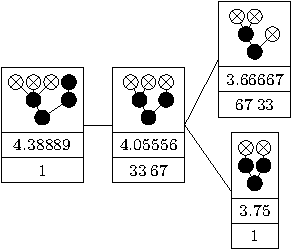
\includegraphics{p3/hlf_not_optimal/001112_hlf_subopt.pdf}
    \caption{Suboptimal HLF run}
  \end{subfigure}
  \begin{subfigure}{.45\linewidth}
    \centering
    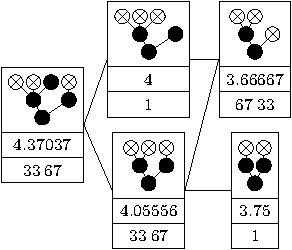
\includegraphics{p3/hlf_not_optimal/001112_hlf_opt.pdf}
    \caption{Optimal HLF run. This is also the overal optimal schedule.}
    \label{fig:hlf-001112-optimal-version}
  \end{subfigure}
  \caption{HLF on $(0,0,1,1,1,2)$. Different runs of HLF do not necessarily produce the same result.}
  \label{fig:hlf-001112}
\end{figure}

This example also reveals that there are several intrees with the profile $\profile{3,2,1}$ that have different optimal run times if scheduled with three processors, namely $(0,0,1,1,2)$ and $(0,0,1,1,1)$.

Because HLF can produce different run times depending which task it has chosen, it is clear that HLF in its raw form can not be optimal. However, note that the optimal schedule for $(0,0,1,1,1,2)$ (shown figure \ref{fig:hlf-001112-optimal-version}) is \emph{one possible HLF-run}. That means that for this intree HLF is not optimal in any case, but the optimal schedule was a particular HLF schedule.

The following section explains that this is not always the case.

\subsection{Examples where HLF is strictly suboptimal}
\label{sec:p3-suboptimal-hlf-strictly-suboptimal}

The example from figure \ref{fig:hlf-001112-optimal-version} shows the optimal run. We observe that this run is a specific instance of HLF, because at each point of time, always tasks with the highest level numbers are chosen.

However, there are intrees, where \emph{no} HLF-run is optimal. Figures \ref{fig:hlf-vs-opt-0012346688}, \ref{fig:hlf-vs-opt-0012446788} and \ref{fig:hlf-vs-opt-00123455799} show some examples for which this is exactly the case.

For these examples, after the first two tasks are finished, the possible remaining intrees are the same for each initial intree, but they are reached with different probabilities. If we inspect the examples and compare the optimal schedule to the HLF schedule, we observe that the HLF schedule has a higher probability to reach a subtree where only \emph{two} tasks can be scheduled, while the optimal schedule has a higher probability to reach snapshots with \emph{three} scheduled tasks. We will later inspect this behaviour in more detail (see section \ref{sec:p3-disproving-long-p3-and-short-p1-time}).

\begin{figure}[ht]
  \centering
  \begin{subfigure}{.45\linewidth}
    \centering
    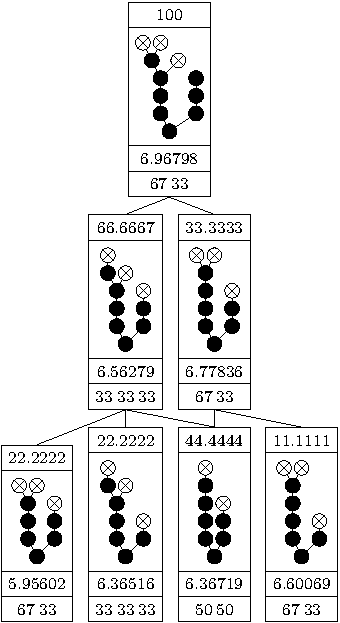
\includegraphics{p3/hlf_not_optimal/0012346688_subopt.pdf}
    \caption{HLF -- suboptimal}
  \end{subfigure}
  \begin{subfigure}{.45\linewidth}
    \centering
    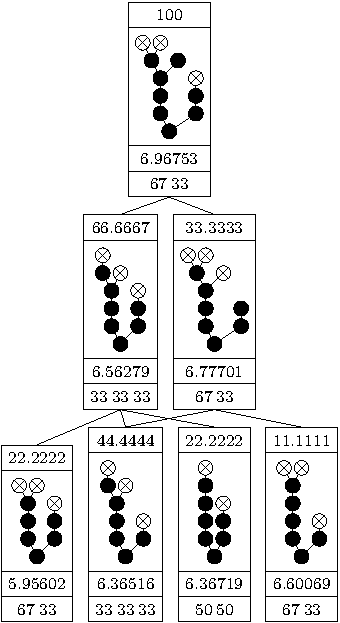
\includegraphics{p3/hlf_not_optimal/0012346688_opt.pdf}
    \caption{Optimal run is non-HLF}
  \end{subfigure}
  \caption{HLF vs. optimal solution for $(0,0,1,2,3,4,6,6,8,8)$}
  \label{fig:hlf-vs-opt-0012346688}
\end{figure}

\begin{figure}[ht]
  \centering
  \begin{subfigure}{.45\linewidth}
    \centering
    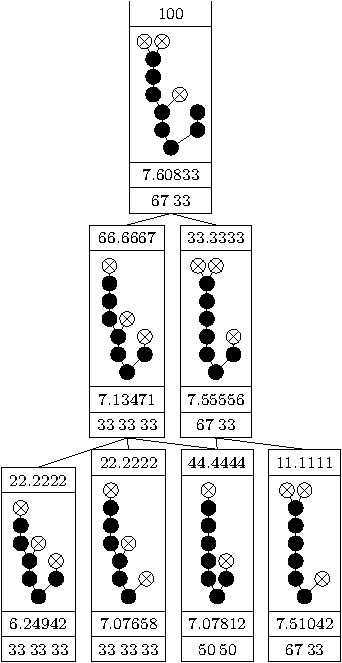
\includegraphics{p3/hlf_not_optimal/0012446788_subopt.pdf}
    \caption{HLF -- suboptimal}
  \end{subfigure}
  \begin{subfigure}{.45\linewidth}
    \centering
    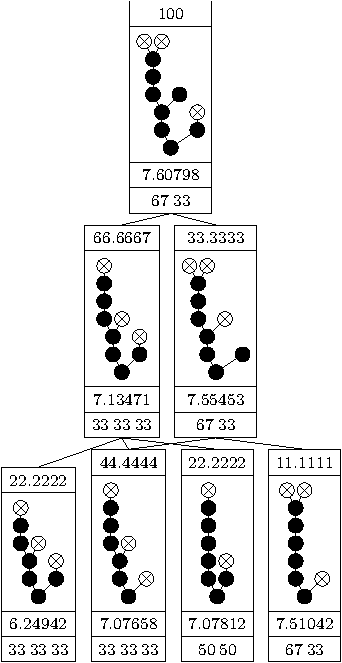
\includegraphics{p3/hlf_not_optimal/0012446788_opt.pdf}
    \caption{Optimal run is non-HLF}
  \end{subfigure}
  \caption{HLF vs. optimal solution for $(0,0,1,2,4,4,6,7,8,8)$ (taken from Ernst Mayr)}
  \label{fig:hlf-vs-opt-0012446788}
\end{figure}
\begin{figure}[ht]
  \centering
  \begin{subfigure}{.45\linewidth}
    \centering
    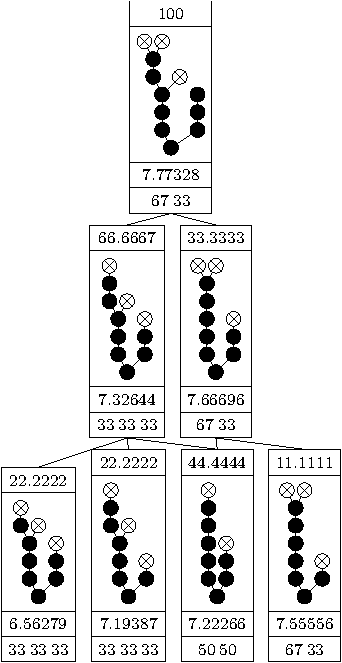
\includegraphics{p3/hlf_not_optimal/00123455799_subopt.pdf}
    \caption{HLF -- suboptimal}
  \end{subfigure}
  \begin{subfigure}{.45\linewidth}
    \centering
    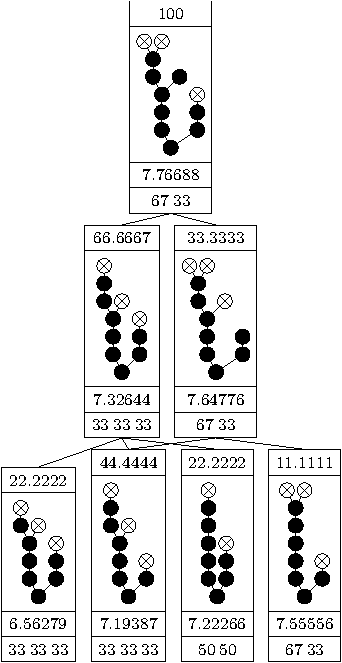
\includegraphics{p3/hlf_not_optimal/00123455799_opt.pdf}
    \caption{Optimal run is non-HLF}
  \end{subfigure}
  \caption{HLF vs. optimal solution for $(0,0,1,2,3,4,5,5,7,9,9)$ (taken from \cite{chandyreynoldsshortpaper1975})}
  \label{fig:hlf-vs-opt-00123455799}
\end{figure}

\subsection{Quality of HLF}
\label{sec:suboptimal-hlf-quality}

We have seen that HLF is suboptimal in some cases, but experience shows that HLF is quite good in many cases. In fact \cite{journals/siamcomp/PapadimitriouT87} have shown the following theorem:

\begin{theorem}
  \label{thm:quality-hlf-papadimitriou}
  There is a function $\beta: \mathbb{N} \mapsto \mathbb{R}^+_0$ with $\lim_{n\rightarrow \infty} \beta(n) = 0$ such that for each intree $I$ and an arbitrary HLF strategy $HLF$ we have
  \begin{equation*}
    T_{HLF}(I) \leq \inf_\pi\, T_{\pi}(I) \cdot \left( 1+\beta(N) \right),
  \end{equation*}
  where $T_{P}(I)$ denotes the expected run time for intree $I$ if it is scheduled by policy $P$, $N$ is the number of tasks in $I$ and the infimum is taken over all scheduling strategies $\pi$.
\end{theorem}

\begin{proof}
  See \cite{journals/siamcomp/PapadimitriouT87}.
\end{proof}

This result is quite useful because it shows that HLF is -- even if not optimal -- quite close as the number of tasks grows. Thus, HLF is probably a good choice in many situations in practice.

Note that theorem \ref{thm:quality-hlf-papadimitriou} states this property for \emph{an arbitrary HLF} strategy, implying that we can use \emph{any} HLF strategy. This in particular means that we do not need to try all possibilities if HLF has several choices.

\subsection{Different categories of sub-optimality}
\label{sec:hlf-suboptimal-two-variants}

As we saw, there are two possibilities for the sub-optimality of HLF:

\begin{itemize}
\item \emph{Not each possible run} of HLF yields the same run time, thus some must be suboptimal.
\item The optimal run has to choose a strict non-HLF task.
\end{itemize}

We use the following nomenclature: A strategy is called \emph{can-optimal} (a term borrowed from \cite{MoritzMaasDiploma}), if it \emph{might} result in an optimal schedule. A strategy that \emph{can not} produce an optimal solution is called \emph{strictly suboptimal} (or simply suboptimmal if it is clear from the context). 

It is a notable fact that there are many cases where HLF is can-optimal. 

We use this distinction to (roughly) differentiate the following strategies into two categories: 

\begin{itemize}
\item The cases where HLF is strictly suboptimal lead us to several strategies that are presented in section \ref{sec:suboptimal-non-hlf-strategies}. These strategies are strict counterparts to HLF.
\item For the cases where HLF is can-optimal, we examined several strategies that try to determine which tasks should be chosen to minimize the expected run time. These strategies are presented in section \ref{sec:suboptimal-hlf-can-optimal-strategies}. These strategies can be seen as ``refinements'' of HLF such that HLF hopefully performs better.
\end{itemize}

We will not only focus on particular strategies, but we will focus on which snapshots can be excluded or which particular structure snapshots might have. That is, the strategies we consider are in many cases ambiguous because they admit several possible choices. However, they do \emph{not} allow \emph{all} possible choices, thereby possibly reducing the amount of snapshots to examine. Not all strategies fall strictly into one of the groups -- we then put it into the category we found more insightful. We derived these new strategies by considering examples of optimal schedules and trying to deduce patterns for them.

Before we start with our own strategies, we do short excurse on why list scheduling can not be optimal.

\section{(Dynamic) list scheduling}
\label{sec:suboptimal-strategies-list-scheduling}

List scheduling considers the structure of the intree and generates a list of tasks sorted in such a way that the tasks that come first in the list shall be priorized and scheduled first, if possible. Static list scheduling does this only once at the beginning of the scheduling process. It is clear that static list scheduling can not be optimal in a general setting because -- depending on which task finishes first -- the next task optimally chosen might vary (see the intree $(0,0,0,2,2,3,5,5,6,6,6)$ in figure \ref{fig:filling-op-is-not-strictly-optimal} for an example).

Dynamic list scheduling priorizes tasks \emph{for each reached subtree}. As shown by \cite{MoritzMaasDiploma}, dynamic list scheduling strategies can not be optimal for non-preemtive scheduling of intrees (whose tasks' run times are exponentially distributed) with three processors.

This can be seen by e.g. examining the intree $(0,0,1,1,1,2,2,2,2,3,6)$\footnote{\emph{Remark:} This is possibly not be the smallest intree for which dynamic list scheduling is suboptimal --- we did not generate it by a program, but derived it manually.} as shown in figure \ref{fig:list-scheduling-counter-example}. Because the subtree shown in figure \ref{fig:list-schedule-counter-example-subtree} is optimally scheduled using other tasks than the one that have to be used when it is reached in the original schedule, there can not exist a dynamic list scheduling strategy that works for \emph{all} intrees.

Note that this also excludes HLF from being optimal.

\begin{figure}[ht]
  \centering
  \begin{subfigure}[b]{.5\textwidth}
    \centering
    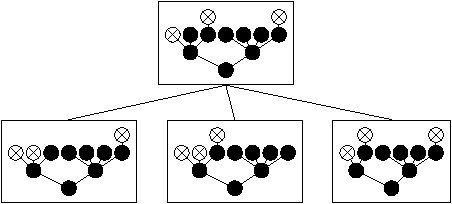
\includegraphics{p3/list_sched_0011122236_opt_sched.pdf}
    \caption{Optimal schedule for intree $(0,0,1,1,1,2,2,2,2,3,6)$. The middle subtree has to be scheduled as shown due to previous choices.}
  \end{subfigure}
  \quad
  \begin{subfigure}[b]{.4\textwidth}
    \centering
    \vfill
    \begin{tikzpicture}[scale=.2]
\node[circle, scale=0.75, fill] (tid0) at (5.25,1.5){};
\node[circle, scale=0.75, fill] (tid1) at (2.25,3){};
\node[circle, scale=0.75, fill] (tid3) at (0.75,4.5){};
\node[circle, scale=0.75, fill] (tid4) at (2.25,4.5){};
\node[circle, scale=0.75, fill] (tid5) at (3.75,4.5){};
\node[circle, scale=0.75, fill, task_scheduled] (tid10) at (3.75,6){};
\draw[](tid5) -- (tid10);
\draw[](tid1) -- (tid3);
\draw[](tid1) -- (tid4);
\draw[](tid1) -- (tid5);
\node[circle, scale=0.75, fill] (tid2) at (7.5,3){};
\node[circle, scale=0.75, fill] (tid6) at (5.25,4.5){};
\node[circle, scale=0.75, fill] (tid7) at (6.75,4.5){};
\node[circle, scale=0.75, fill, task_scheduled] (tid8) at (8.25,4.5){};
\node[circle, scale=0.75, fill, task_scheduled] (tid9) at (9.75,4.5){};
\draw[](tid2) -- (tid6);
\draw[](tid2) -- (tid7);
\draw[](tid2) -- (tid8);
\draw[](tid2) -- (tid9);
\draw[](tid0) -- (tid1);
\draw[](tid0) -- (tid2);
\end{tikzpicture}

%%% Local Variables:
%%% TeX-master: "thesis/thesis.tex"
%%% End: 

    \vfill
    \caption{This subtree of $(0,0,1,1,1,2,2,2,3,6)$ is optimally scheduled as shown, but in the optimal schedule for the original intree, it has to be scheduled in another way.}
    \label{fig:list-schedule-counter-example-subtree}
  \end{subfigure}
  \caption{A counterexample for list scheduling}
  \label{fig:list-scheduling-counter-example}
\end{figure}

That is, an optimal strategy has to consider which tasks are already scheduled from previous steps and can not rely \emph{only} on the current intree's structure. We experience this phenomenon in many intrees shown in this chapter. However, for the initial snapshot, we -- of course -- \emph{must} rely on the structure of the intree. Thus, we will examine some strategies and inspect if the first snapshot of an optimal schedule adheres specific rules.

\section{Non-HLF strategies}
\label{sec:suboptimal-non-hlf-strategies}

We saw in section \ref{sec:hlf-p3-suboptimal} that there are examples where HLF is strictly suboptimal. We now present some strategies that we took into consideration and that we examined w.r.t. their optimality. 

We therefore considered optimal schedules and examined whether the initial snapshot (i.e. the initial choice of tasks) are formed upon a certain pattern.

These strategies are strongly different from HLF and rely upon the structure of the intree. None of the strategies considered lead us to strictly optimal results in all cases.

\subsection{``2-HLF plus 1''}
\label{sec:disproving-2hlf-plus-1}

We examined all intrees with up to 13 tasks, especially the cases where HLF is not optimal. Thereby, we obsered that in all cases where three tasks could be scheduled, the optimal solution scheduled two tasks that could be chosen by HLF for two processors and \emph{only the third} task \emph{might} be a task that would not have been chosen by HLF (see figures \ref{fig:hlf-vs-opt-0012346688}, \ref{fig:hlf-vs-opt-0012446788} and \ref{fig:hlf-vs-opt-00123455799} as particular instances of those). Thus, we examined whether an optimal scheduling strategy for three processors has always \emph{at most one} task that is non-HLF. Interestingly, there is an intree with 14 tasks, whose optimal schedule starts out by choosing the single topmost task and \emph{two} non-HLF tasks. This intree (its sequence is $(0,0,1,2,2,3,3,6,8,9,10,11,12)$) is shown in figure \ref{fig:2-hlf-plus-one-not-optimal}. One can possibly generalize this intree to a whole family of intrees where the optimal strategy initially chooses the single topmost task, and two lowest-level leaves by adding leaves along the longest chain. This results in intrees of the form $(0, 0, 1, 2, 3, 4, 4, 5, 5, 8, 10, 11, 12, 13, 14, 15,\dots)$.

\begin{figure}[ht]
  \centering
  \begin{subfigure}{.5\textwidth}
    \centering
    \renewcommand{\leveltopI}{-22cm + \leveltop}
\renewcommand{\leveltopII}{-22cm + \leveltopI}
\renewcommand{\leveltopIII}{-22cm + \leveltopII}
\renewcommand{\leveltopIIII}{-22cm + \leveltopIII}
\renewcommand{\leveltopIIIII}{-22cm + \leveltopIIII}
\renewcommand{\leveltopIIIIII}{-22cm + \leveltopIIIII}
\renewcommand{\leveltopIIIIIII}{-22cm + \leveltopIIIIII}
\renewcommand{\leveltopIIIIIIII}{-22cm + \leveltopIIIIIII}
\renewcommand{\leveltopIIIIIIIII}{-22cm + \leveltopIIIIIIII}
\renewcommand{\leveltopIIIIIIIIII}{-22cm + \leveltopIIIIIIIII}
\renewcommand{\leveltopIIIIIIIIIII}{-22cm + \leveltopIIIIIIIIII}
\renewcommand{\leveltopIIIIIIIIIIII}{-22cm + \leveltopIIIIIIIIIII}
\renewcommand{\leveltopIIIIIIIIIIIII}{-22cm + \leveltopIIIIIIIIIIII}
\renewcommand{\leveltopIIIIIIIIIIIIII}{-22cm + \leveltopIIIIIIIIIIIII}
\begin{tikzpicture}[scale=.2, anchor=south]
\begin{scope}[yshift=\leveltopI cm]
\matrix (line1)[column sep=0.25cm] {
\node[draw=black, rectangle split,  rectangle split parts=3] (sn0x88074b8){
\begin{tikzpicture}[scale=.2]
\node[circle, scale=0.75, fill] (tid0) at (3,1.5){};
\node[circle, scale=0.75, fill] (tid1) at (1.5,3){};
\node[circle, scale=0.75, fill, task_scheduled] (tid3) at (0.75,4.5){};
\node[circle, scale=0.75, fill] (tid4) at (2.25,4.5){};
\draw[](tid1) -- (tid3);
\draw[](tid1) -- (tid4);
\node[circle, scale=0.75, fill] (tid2) at (4.5,3){};
\node[circle, scale=0.75, fill] (tid5) at (4.5,4.5){};
\node[circle, scale=0.75, fill, task_scheduled] (tid6) at (3.75,6){};
\node[circle, scale=0.75, fill] (tid7) at (5.25,6){};
\node[circle, scale=0.75, fill] (tid8) at (5.25,7.5){};
\node[circle, scale=0.75, fill] (tid9) at (5.25,9){};
\node[circle, scale=0.75, fill] (tid10) at (5.25,10.5){};
\node[circle, scale=0.75, fill] (tid11) at (5.25,12){};
\node[circle, scale=0.75, fill] (tid12) at (5.25,13.5){};
\node[circle, scale=0.75, fill, task_scheduled] (tid13) at (5.25,15){};
\draw[](tid12) -- (tid13);
\draw[](tid11) -- (tid12);
\draw[](tid10) -- (tid11);
\draw[](tid9) -- (tid10);
\draw[](tid8) -- (tid9);
\draw[](tid7) -- (tid8);
\draw[](tid5) -- (tid6);
\draw[](tid5) -- (tid7);
\draw[](tid2) -- (tid5);
\draw[](tid0) -- (tid1);
\draw[](tid0) -- (tid2);
\end{tikzpicture}
\nodepart{two}
\footnotesize{10.03552}
\nodepart{three}
\footnotesize{$33\:33\:33$}
};
 & 
\\
};
\end{scope}
\begin{scope}[yshift=\leveltopII cm]
\matrix (line2)[column sep=0.25cm] {
\node[draw=black, rectangle split,  rectangle split parts=3] (sn0x88073a0){
\begin{tikzpicture}[scale=.2]
\node[circle, scale=0.75, fill] (tid0) at (3,1.5){};
\node[circle, scale=0.75, fill] (tid1) at (1.5,3){};
\node[circle, scale=0.75, fill, task_scheduled] (tid3) at (0.75,4.5){};
\node[circle, scale=0.75, fill] (tid4) at (2.25,4.5){};
\draw[](tid1) -- (tid3);
\draw[](tid1) -- (tid4);
\node[circle, scale=0.75, fill] (tid2) at (4.5,3){};
\node[circle, scale=0.75, fill] (tid5) at (4.5,4.5){};
\node[circle, scale=0.75, fill, task_scheduled] (tid6) at (3.75,6){};
\node[circle, scale=0.75, fill] (tid7) at (5.25,6){};
\node[circle, scale=0.75, fill] (tid8) at (5.25,7.5){};
\node[circle, scale=0.75, fill] (tid9) at (5.25,9){};
\node[circle, scale=0.75, fill] (tid10) at (5.25,10.5){};
\node[circle, scale=0.75, fill] (tid11) at (5.25,12){};
\node[circle, scale=0.75, fill, task_scheduled] (tid12) at (5.25,13.5){};
\draw[](tid11) -- (tid12);
\draw[](tid10) -- (tid11);
\draw[](tid9) -- (tid10);
\draw[](tid8) -- (tid9);
\draw[](tid7) -- (tid8);
\draw[](tid5) -- (tid6);
\draw[](tid5) -- (tid7);
\draw[](tid2) -- (tid5);
\draw[](tid0) -- (tid1);
\draw[](tid0) -- (tid2);
\end{tikzpicture}
\nodepart{two}
\footnotesize{9.06481}
\nodepart{three}
\footnotesize{$33\:33\:33$}
};
 & 
\node[draw=black, rectangle split,  rectangle split parts=3] (sn0x88048e8){
\begin{tikzpicture}[scale=.2]
\node[circle, scale=0.75, fill] (tid0) at (2.25,1.5){};
\node[circle, scale=0.75, fill] (tid1) at (0.75,3){};
\node[circle, scale=0.75, fill, task_scheduled] (tid3) at (0.75,4.5){};
\draw[](tid1) -- (tid3);
\node[circle, scale=0.75, fill] (tid2) at (3,3){};
\node[circle, scale=0.75, fill] (tid4) at (3,4.5){};
\node[circle, scale=0.75, fill, task_scheduled] (tid5) at (2.25,6){};
\node[circle, scale=0.75, fill] (tid6) at (3.75,6){};
\node[circle, scale=0.75, fill] (tid7) at (3.75,7.5){};
\node[circle, scale=0.75, fill] (tid8) at (3.75,9){};
\node[circle, scale=0.75, fill] (tid9) at (3.75,10.5){};
\node[circle, scale=0.75, fill] (tid10) at (3.75,12){};
\node[circle, scale=0.75, fill] (tid11) at (3.75,13.5){};
\node[circle, scale=0.75, fill, task_scheduled] (tid12) at (3.75,15){};
\draw[](tid11) -- (tid12);
\draw[](tid10) -- (tid11);
\draw[](tid9) -- (tid10);
\draw[](tid8) -- (tid9);
\draw[](tid7) -- (tid8);
\draw[](tid6) -- (tid7);
\draw[](tid4) -- (tid5);
\draw[](tid4) -- (tid6);
\draw[](tid2) -- (tid4);
\draw[](tid0) -- (tid1);
\draw[](tid0) -- (tid2);
\end{tikzpicture}
\nodepart{two}
\footnotesize{10.0202}
\nodepart{three}
\footnotesize{$33\:33\:33$}
};
 & 
\node[draw=black, rectangle split,  rectangle split parts=3] (sn0x8805800){
\begin{tikzpicture}[scale=.2]
\node[circle, scale=0.75, fill] (tid0) at (2.25,1.5){};
\node[circle, scale=0.75, fill] (tid1) at (1.5,3){};
\node[circle, scale=0.75, fill, task_scheduled] (tid3) at (0.75,4.5){};
\node[circle, scale=0.75, fill, task_scheduled] (tid4) at (2.25,4.5){};
\draw[](tid1) -- (tid3);
\draw[](tid1) -- (tid4);
\node[circle, scale=0.75, fill] (tid2) at (3.75,3){};
\node[circle, scale=0.75, fill] (tid5) at (3.75,4.5){};
\node[circle, scale=0.75, fill] (tid6) at (3.75,6){};
\node[circle, scale=0.75, fill] (tid7) at (3.75,7.5){};
\node[circle, scale=0.75, fill] (tid8) at (3.75,9){};
\node[circle, scale=0.75, fill] (tid9) at (3.75,10.5){};
\node[circle, scale=0.75, fill] (tid10) at (3.75,12){};
\node[circle, scale=0.75, fill] (tid11) at (3.75,13.5){};
\node[circle, scale=0.75, fill, task_scheduled] (tid12) at (3.75,15){};
\draw[](tid11) -- (tid12);
\draw[](tid10) -- (tid11);
\draw[](tid9) -- (tid10);
\draw[](tid8) -- (tid9);
\draw[](tid7) -- (tid8);
\draw[](tid6) -- (tid7);
\draw[](tid5) -- (tid6);
\draw[](tid2) -- (tid5);
\draw[](tid0) -- (tid1);
\draw[](tid0) -- (tid2);
\end{tikzpicture}
\nodepart{two}
\footnotesize{10.0215}
\nodepart{three}
\footnotesize{$33\:67$}
};
 & 
\\
};
\end{scope}
\begin{scope}[yshift=\leveltopIII cm]
\matrix (line3)[column sep=0.25cm] {
\node[draw=black, rectangle split,  rectangle split parts=3] (sn0x88072b8){
\begin{tikzpicture}[scale=.2]
\node[circle, scale=0.75, fill] (tid0) at (3,1.5){};
\node[circle, scale=0.75, fill] (tid1) at (1.5,3){};
\node[circle, scale=0.75, fill, task_scheduled] (tid3) at (0.75,4.5){};
\node[circle, scale=0.75, fill] (tid4) at (2.25,4.5){};
\draw[](tid1) -- (tid3);
\draw[](tid1) -- (tid4);
\node[circle, scale=0.75, fill] (tid2) at (4.5,3){};
\node[circle, scale=0.75, fill] (tid5) at (4.5,4.5){};
\node[circle, scale=0.75, fill, task_scheduled] (tid6) at (3.75,6){};
\node[circle, scale=0.75, fill] (tid7) at (5.25,6){};
\node[circle, scale=0.75, fill] (tid8) at (5.25,7.5){};
\node[circle, scale=0.75, fill] (tid9) at (5.25,9){};
\node[circle, scale=0.75, fill] (tid10) at (5.25,10.5){};
\node[circle, scale=0.75, fill, task_scheduled] (tid11) at (5.25,12){};
\draw[](tid10) -- (tid11);
\draw[](tid9) -- (tid10);
\draw[](tid8) -- (tid9);
\draw[](tid7) -- (tid8);
\draw[](tid5) -- (tid6);
\draw[](tid5) -- (tid7);
\draw[](tid2) -- (tid5);
\draw[](tid0) -- (tid1);
\draw[](tid0) -- (tid2);
\end{tikzpicture}
\nodepart{two}
\footnotesize{8.11701}
\nodepart{three}
\footnotesize{$33\:33\:33$}
};
 & 
\node[draw=black, rectangle split,  rectangle split parts=3] (sn0x88047c8){
\begin{tikzpicture}[scale=.2]
\node[circle, scale=0.75, fill] (tid0) at (2.25,1.5){};
\node[circle, scale=0.75, fill] (tid1) at (0.75,3){};
\node[circle, scale=0.75, fill, task_scheduled] (tid3) at (0.75,4.5){};
\draw[](tid1) -- (tid3);
\node[circle, scale=0.75, fill] (tid2) at (3,3){};
\node[circle, scale=0.75, fill] (tid4) at (3,4.5){};
\node[circle, scale=0.75, fill, task_scheduled] (tid5) at (2.25,6){};
\node[circle, scale=0.75, fill] (tid6) at (3.75,6){};
\node[circle, scale=0.75, fill] (tid7) at (3.75,7.5){};
\node[circle, scale=0.75, fill] (tid8) at (3.75,9){};
\node[circle, scale=0.75, fill] (tid9) at (3.75,10.5){};
\node[circle, scale=0.75, fill] (tid10) at (3.75,12){};
\node[circle, scale=0.75, fill, task_scheduled] (tid11) at (3.75,13.5){};
\draw[](tid10) -- (tid11);
\draw[](tid9) -- (tid10);
\draw[](tid8) -- (tid9);
\draw[](tid7) -- (tid8);
\draw[](tid6) -- (tid7);
\draw[](tid4) -- (tid5);
\draw[](tid4) -- (tid6);
\draw[](tid2) -- (tid4);
\draw[](tid0) -- (tid1);
\draw[](tid0) -- (tid2);
\end{tikzpicture}
\nodepart{two}
\footnotesize{9.03829}
\nodepart{three}
\footnotesize{$33\:33\:33$}
};
 & 
\node[draw=black, rectangle split,  rectangle split parts=3] (sn0x88056e0){
\begin{tikzpicture}[scale=.2]
\node[circle, scale=0.75, fill] (tid0) at (2.25,1.5){};
\node[circle, scale=0.75, fill] (tid1) at (1.5,3){};
\node[circle, scale=0.75, fill, task_scheduled] (tid3) at (0.75,4.5){};
\node[circle, scale=0.75, fill, task_scheduled] (tid4) at (2.25,4.5){};
\draw[](tid1) -- (tid3);
\draw[](tid1) -- (tid4);
\node[circle, scale=0.75, fill] (tid2) at (3.75,3){};
\node[circle, scale=0.75, fill] (tid5) at (3.75,4.5){};
\node[circle, scale=0.75, fill] (tid6) at (3.75,6){};
\node[circle, scale=0.75, fill] (tid7) at (3.75,7.5){};
\node[circle, scale=0.75, fill] (tid8) at (3.75,9){};
\node[circle, scale=0.75, fill] (tid9) at (3.75,10.5){};
\node[circle, scale=0.75, fill] (tid10) at (3.75,12){};
\node[circle, scale=0.75, fill, task_scheduled] (tid11) at (3.75,13.5){};
\draw[](tid10) -- (tid11);
\draw[](tid9) -- (tid10);
\draw[](tid8) -- (tid9);
\draw[](tid7) -- (tid8);
\draw[](tid6) -- (tid7);
\draw[](tid5) -- (tid6);
\draw[](tid2) -- (tid5);
\draw[](tid0) -- (tid1);
\draw[](tid0) -- (tid2);
\end{tikzpicture}
\nodepart{two}
\footnotesize{9.03914}
\nodepart{three}
\footnotesize{$33\:67$}
};
 & 
\node[draw=black, rectangle split,  rectangle split parts=3] (sn0x88033c8){
\begin{tikzpicture}[scale=.2]
\node[circle, scale=0.75, fill] (tid0) at (2.25,1.5){};
\node[circle, scale=0.75, fill, task_scheduled] (tid1) at (0.75,3){};
\node[circle, scale=0.75, fill] (tid2) at (3,3){};
\node[circle, scale=0.75, fill] (tid3) at (3,4.5){};
\node[circle, scale=0.75, fill, task_scheduled] (tid4) at (2.25,6){};
\node[circle, scale=0.75, fill] (tid5) at (3.75,6){};
\node[circle, scale=0.75, fill] (tid6) at (3.75,7.5){};
\node[circle, scale=0.75, fill] (tid7) at (3.75,9){};
\node[circle, scale=0.75, fill] (tid8) at (3.75,10.5){};
\node[circle, scale=0.75, fill] (tid9) at (3.75,12){};
\node[circle, scale=0.75, fill] (tid10) at (3.75,13.5){};
\node[circle, scale=0.75, fill, task_scheduled] (tid11) at (3.75,15){};
\draw[](tid10) -- (tid11);
\draw[](tid9) -- (tid10);
\draw[](tid8) -- (tid9);
\draw[](tid7) -- (tid8);
\draw[](tid6) -- (tid7);
\draw[](tid5) -- (tid6);
\draw[](tid3) -- (tid4);
\draw[](tid3) -- (tid5);
\draw[](tid2) -- (tid3);
\draw[](tid0) -- (tid1);
\draw[](tid0) -- (tid2);
\end{tikzpicture}
\nodepart{two}
\footnotesize{10.0097}
\nodepart{three}
\footnotesize{$33\:33\:33$}
};
 & 
\node[draw=black, rectangle split,  rectangle split parts=3] (sn0x8803e80){
\begin{tikzpicture}[scale=.2]
\node[circle, scale=0.75, fill] (tid0) at (1.5,1.5){};
\node[circle, scale=0.75, fill] (tid1) at (0.75,3){};
\node[circle, scale=0.75, fill, task_scheduled] (tid3) at (0.75,4.5){};
\draw[](tid1) -- (tid3);
\node[circle, scale=0.75, fill] (tid2) at (2.25,3){};
\node[circle, scale=0.75, fill] (tid4) at (2.25,4.5){};
\node[circle, scale=0.75, fill] (tid5) at (2.25,6){};
\node[circle, scale=0.75, fill] (tid6) at (2.25,7.5){};
\node[circle, scale=0.75, fill] (tid7) at (2.25,9){};
\node[circle, scale=0.75, fill] (tid8) at (2.25,10.5){};
\node[circle, scale=0.75, fill] (tid9) at (2.25,12){};
\node[circle, scale=0.75, fill] (tid10) at (2.25,13.5){};
\node[circle, scale=0.75, fill, task_scheduled] (tid11) at (2.25,15){};
\draw[](tid10) -- (tid11);
\draw[](tid9) -- (tid10);
\draw[](tid8) -- (tid9);
\draw[](tid7) -- (tid8);
\draw[](tid6) -- (tid7);
\draw[](tid5) -- (tid6);
\draw[](tid4) -- (tid5);
\draw[](tid2) -- (tid4);
\draw[](tid0) -- (tid1);
\draw[](tid0) -- (tid2);
\end{tikzpicture}
\nodepart{two}
\footnotesize{10.0127}
\nodepart{three}
\footnotesize{$50\:50$}
};
 & 
\\
};
\end{scope}
\draw (sn0x88074b8.south) -- (sn0x88048e8.north);
\draw (sn0x88074b8.south) -- (sn0x8805800.north);
\draw (sn0x88074b8.south) -- (sn0x88073a0.north);
\draw (sn0x88073a0.south) -- (sn0x88047c8.north);
\draw (sn0x88073a0.south) -- (sn0x88056e0.north);
\draw (sn0x88073a0.south) -- (sn0x88072b8.north);
\draw (sn0x88048e8.south) -- (sn0x88033c8.north);
\draw (sn0x88048e8.south) -- (sn0x8803e80.north);
\draw (sn0x88048e8.south) -- (sn0x88047c8.north);
\draw (sn0x8805800.south) -- (sn0x8803e80.north);
\draw (sn0x8805800.south) -- (sn0x88056e0.north);
\end{tikzpicture}
%%% Local Variables:
%%% TeX-master: "thesis/thesis.tex"
%%% End: 

    \caption{HLF-Schedule}
  \end{subfigure}
  \quad
  \begin{subfigure}{.40\textwidth}
    \centering
    \renewcommand{\leveltopI}{-16cm + \leveltop}
\renewcommand{\leveltopII}{-16cm + \leveltopI}
\renewcommand{\leveltopIII}{-16cm + \leveltopII}
\renewcommand{\leveltopIIII}{-16cm + \leveltopIII}
\renewcommand{\leveltopIIIII}{-16cm + \leveltopIIII}
\renewcommand{\leveltopIIIIII}{-16cm + \leveltopIIIII}
\renewcommand{\leveltopIIIIIII}{-16cm + \leveltopIIIIII}
\renewcommand{\leveltopIIIIIIII}{-16cm + \leveltopIIIIIII}
\renewcommand{\leveltopIIIIIIIII}{-16cm + \leveltopIIIIIIII}
\renewcommand{\leveltopIIIIIIIIII}{-16cm + \leveltopIIIIIIIII}
\renewcommand{\leveltopIIIIIIIIIII}{-16cm + \leveltopIIIIIIIIII}
\renewcommand{\leveltopIIIIIIIIIIII}{-16cm + \leveltopIIIIIIIIIII}
\renewcommand{\leveltopIIIIIIIIIIIII}{-16cm + \leveltopIIIIIIIIIIII}
\renewcommand{\leveltopIIIIIIIIIIIIII}{-16cm + \leveltopIIIIIIIIIIIII}
\begin{tikzpicture}[scale=.2, anchor=south]
\begin{scope}[yshift=\leveltopI cm]
\matrix (line1)[column sep=0.5cm] {
\node[draw=black, rectangle split,  rectangle split parts=2] (sn0x87252b0){
\begin{tikzpicture}[scale=.2]
\node[circle, scale=0.75, fill] (tid0) at (3,1.5){};
\node[circle, scale=0.75, fill] (tid1) at (1.5,3){};
\node[circle, scale=0.75, fill, task_scheduled] (tid3) at (0.75,4.5){};
\node[circle, scale=0.75, fill, task_scheduled] (tid4) at (2.25,4.5){};
\draw[](tid1) -- (tid3);
\draw[](tid1) -- (tid4);
\node[circle, scale=0.75, fill] (tid2) at (4.5,3){};
\node[circle, scale=0.75, fill] (tid5) at (4.5,4.5){};
\node[circle, scale=0.75, fill] (tid6) at (3.75,6){};
\node[circle, scale=0.75, fill] (tid7) at (5.25,6){};
\node[circle, scale=0.75, fill] (tid8) at (5.25,7.5){};
\node[circle, scale=0.75, fill] (tid9) at (5.25,9){};
\node[circle, scale=0.75, fill] (tid10) at (5.25,10.5){};
\node[circle, scale=0.75, fill] (tid11) at (5.25,12){};
\node[circle, scale=0.75, fill] (tid12) at (5.25,13.5){};
\node[circle, scale=0.75, fill, task_scheduled] (tid13) at (5.25,15){};
\draw[](tid12) -- (tid13);
\draw[](tid11) -- (tid12);
\draw[](tid10) -- (tid11);
\draw[](tid9) -- (tid10);
\draw[](tid8) -- (tid9);
\draw[](tid7) -- (tid8);
\draw[](tid5) -- (tid6);
\draw[](tid5) -- (tid7);
\draw[](tid2) -- (tid5);
\draw[](tid0) -- (tid1);
\draw[](tid0) -- (tid2);
\end{tikzpicture}
\nodepart{two}
\footnotesize{10.03547}
};
\\
};
\end{scope}
\end{tikzpicture}
%%% Local Variables:
%%% TeX-master: "thesis/thesis.tex"
%%% End: 

    \caption{Optimal schedule picking \emph{two} non-HLF tasks.}
  \end{subfigure}
  \caption{Intree $(0,0,1,2,2,3,3,6,8,9,10,11,12)$ requires the optimal schedule to start out by choosing two non-HLF tasks.}
  \label{fig:2-hlf-plus-one-not-optimal}
\end{figure}

\subsection{Only highest or lowest leaves}
\label{sec:disproving-only-highest-or-lowest-leaves}

The trees we examined so far resulted in schedules that picked only combinations \emph{highest leaves and lowest leaves} possible. Thus, we were tempted to think that an optimal schedule chooses only topmost tasks or leaves whose level is minimal (among all leaves). However, this is not a criterion for an optimal schedule, as we can observe by scheduling the 13-tasks-intree $(0,0,0,2,3,4,5,7,7,9,10,10)$, which is shown in figure \ref{fig:only-high-or-low-not-optimal}. For this intree, we have to schedule two topmost tasks and one task on level 3, but there is one unscheduled task remaining on level 1.

\begin{figure}[ht]
  \centering
  \begin{subfigure}{.45\textwidth}
    \centering
    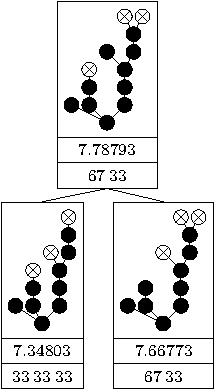
\includegraphics{p3/only_high_or_low/00023457791010_opt.pdf}
    \caption{Optimal schedule picking a non-HLF task that is also not the lowest possible.}
  \end{subfigure}
  \quad
  \begin{subfigure}{.45\textwidth}
    \centering
    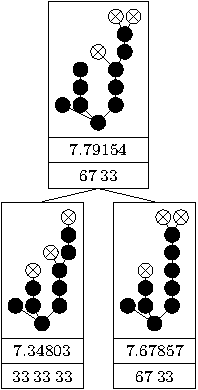
\includegraphics{p3/only_high_or_low/00023457791010_subopt.pdf}
    \caption{Suboptimal HLF-Schedule.}
  \end{subfigure}
  \caption{Intree $(0,0,0,2,3,4,5,7,7,9,10,10)$ shows that there are intrees where an optimal schedule has to choose a non-HLF task that has a higher level than some non-chosen task.}
  \label{fig:only-high-or-low-not-optimal}
\end{figure}

\section{Refining can-optimal HLF}
\label{sec:suboptimal-hlf-can-optimal-strategies}

As mentioned in section \ref{sec:hlf-suboptimal-two-variants}, there are many cases where HLF is \emph{can-optimal}, i.e. where the optimal schedule always has tasks of the highest levels scheduled, but not each HLF schedule is optimal. This results from situations where HLF can choose one from several task as the next task to be scheduled. We describe some strategies that try to eliminate these ambiguities and give counterexamples that show that these strategies are not optimal.

\subsection{``As few free paths as possible''}
\label{sec:disproving-hlf-no-free-chain}

(For now,) we call a path from the root to a leaf (i.e. a ready task) $t$ \emph{free} if no task along this path except the root has a scheduled predecessor.

One might be tempted to think that it should be the foremost goal to exploit parallelism as good as possible and that this might be acchieved by choosing the currently scheduled tasks in a manner such that there are as few free paths as possible in an optimal schedule. That is, we choose the leaves in a way so that the ends of as many different paths as possible are scheduled. This strategy was the first that came to our mind and was inspired by looking at the counterexamples against HLF depicted in figures \ref{fig:hlf-001112}, \ref{fig:hlf-vs-opt-0012346688}, \ref{fig:hlf-vs-opt-0012446788} and \ref{fig:hlf-vs-opt-00123455799}, where we had no free paths in an optimal schedule, but one free path in the suboptimal (possibly non-HLF) schedule. %We observe for these intrees that the optimal schedules has no as few free chains as possible.

However, there are examples where the optimal schedule contains snapshots that do not adhere this property. Consider e.g. the tree $(0,0,0,1,1,1,2,2,3)$ (figure \ref{fig:hlfnfc-is-not-optimal} compares the optimal schedule to the no-free-paths schedule).

\begin{figure}[ht]
  \centering
  \begin{subfigure}{.45\textwidth}
    \centering
    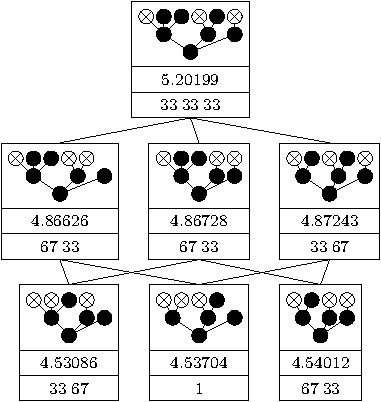
\includegraphics{p3/hlfnfc_not_optimal/000111223_hlfnfc.pdf}
    \caption{HLF schedule while choosing tasks such that there are as few free paths as possible (in this case 0) -- overall run time of 5.20199.}
  \end{subfigure}
  \quad
  \begin{subfigure}{.45\textwidth}
    \centering
    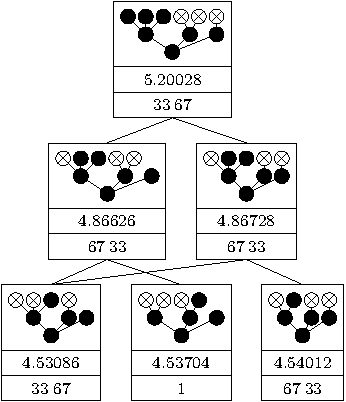
\includegraphics{p3/hlfnfc_not_optimal/000111223_opt.pdf}
    \caption{Optimal schedule (run time 5.20028) has three free paths at the beginning.}
  \end{subfigure}
  \caption{HLF with as few free paths as possible is not necessarily optimal.}
  \label{fig:hlfnfc-is-not-optimal}
\end{figure}

\subsection{Subtree with minimum number of topmost tasks}
\label{sec:suboptimal-hlf-can-optimal-subtree-fewest-toptasks}

If we consider the intree $(0,0,0,1,1,1,2,2,3)$, we see that an optimal schedule picks 7,8 and 9 as initially scheduled tasks (see figure \ref{fig:hlfnfc-is-not-optimal}). Moreover, in many cases, topmost-tasks that are the \emph{single direct predecessor} of their respective direct successor, are chosen by an optimal schedule.

These facts lead us to the suspicion that -- if we have an intree for which HLF is can-optimal -- (informally) we should prefer ready tasks in the subtrees with the lowest number of topmost tasks. 

In this context, it is important to exactly describe which subtree we are talking about. Therefore, we employ the following definition:

\begin{definition}[Topmost-maximal subtree for a leaf]
  Let $t$ be a leaf of an intree $I$ and let $p=(t, t_1, t_2, t_3, \dots, r)$ be the path from $t$ to the root $r$.

  The \emph{topmost-maximal subtree for a leaf} $t$ is the subtree rooted at the \emph{lowest} task $t^*$ within $p$ different from $t$ and that does \emph{not} contain more topmost tasks than the subtree\footnote{Please note that in this definition we do not require the subtrees to contain the root.} rooted at the direct successor of $t$. %predecessor of $t^*$ within $p$.
\end{definition}

As an example, consider the following intree (remember that topmost tasks are defined to be the tasks whose levels are at least as large as the level of \emph{any} task in the intree --- see section \ref{sec:foundations-graph-theory}):

\begin{center}
  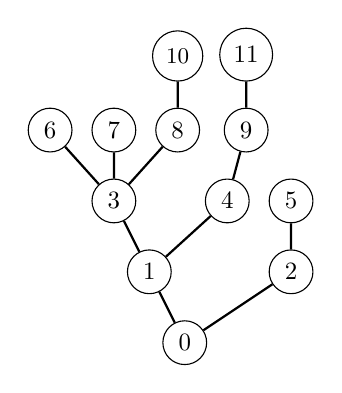
\begin{tikzpicture}[scale=.6, anchor=south]
    \node[circle, scale=0.9, draw] (tid0) at (3,1.5){0};
    \node[circle, scale=0.9, draw] (tid1) at (2.25,3){1};
    \node[circle, scale=0.9, draw] (tid2) at (1.5,4.5){3};
    \node[circle, scale=0.9, draw] (tid7) at (0.15,6){6};
    \node[circle, scale=0.9, draw] (tid10) at (1.5,6){7};
    \draw[ thick](tid2) -- (tid7);
    \draw[ thick](tid2) -- (tid10);
    \node[circle, scale=0.9, draw] (tid3) at (3.9,4.5){4};
    \node[circle, scale=0.9, draw] (tid5) at (2.85,6){8};
    \node[circle, scale=0.9, draw] (tid6) at (2.85,7.5){\small 10};
    \draw[ thick](tid5) -- (tid6);
    \draw[ thick](tid2) -- (tid5);
    \draw[ thick](tid1) -- (tid2);
    \draw[ thick](tid1) -- (tid3);
    \node[circle, scale=0.9, draw] (tid4) at (5.25,3){2};
    \node[circle, scale=0.9, draw] (tid9) at (4.3,6){9};
    \draw[ thick](tid3) -- (tid9);
    \node[circle, scale=0.9, draw] (tid11) at (4.3,7.5){11};
    \draw[ thick](tid11) -- (tid9);
    \node[circle, scale=0.9, draw] (tid8) at (5.25,4.5){5};
    \draw[ thick](tid4) -- (tid8);
    \draw[ thick](tid0) -- (tid1);
    \draw[ thick](tid0) -- (tid4);
  \end{tikzpicture}
\end{center}

The topmost-maximal subtree for leaf 10 is the subtree rooted at node 3, which can be derived as follows:
\begin{itemize}
\item The path from 10 to the root 0 is given by $p=(10,8,3,1,0)$.
\item The successor of 10 is 8, and the subtree rooted at task 8 (called $I_8$) contains exactly one topmost task, namely 10. Thus, we have to find the lowest task whose subtree has not more than 1 topmost task.
\item We consider the subtrees rooted at the tasks along this path, and denote the subtree rooted at node $x$ by $I_x$:
  \begin{itemize}
  \item The subtree rooted at 10 (called $I_{10}$) contains only the topmost task 10. It is omitted because we want to find the lowest task along the path that is different from 10.
  \item Subtree $I_8$ contains only topmost task 10.
  \item Subtree $I_3$ still contains only 10 as the topmost task (it introduces only new \emph{leaves}, namely 6 and 7).
  \item Subtree $I_1$ contains 10 \emph{and} 11 as topmost tasks.
  \end{itemize}
\item As seen, task 3 is the lowest task within $p$ that does not contain more topmost tasks than $I_8$.
\end{itemize}

A strategy for cases where HLF is can-optimal now might be to resolve HLF-ambiguities as follows:
\begin{itemize}
\item Generate all possible choices that could result from HLF.
\item For each topmost task, compute the topmost-maximal subtree.
\item Prefer choices of topmost tasks where the topmost-maximal subtrees contain fewer topmost tasks.
\end{itemize}

%The last step in the above explanation can be viewed as follows: We first create all possible choices of topmost tasks and then only pursue those, where there is no topmost-maximal subtree that has unscheduled topmost tasks.

This strategy seems to do a good job in many cases, but can be seen to be false by examining the optimal schedule for the following intree with 11 tasks: $(0,0,1,2,2,2,3,3,3,4)$. It is shown in figure \ref{fig:subtree-with-fewest-toptasks-suboptimal}.

\emph{Remark:} We did not specify what should be done if there are several maximal subtrees with the same number of topmost tasks, but our counterexample suffices that this strategy does not work optimally even if there are no maximal subtrees with the same number of nodes. 

Beyond this, The tree $(0,0,1,2,2,2,3,3,3,4)$ in particular shows that there are situations where a topmost task that is the \emph{single} requirement for its successor is initially \emph{not} scheduled in the optimal case. During our research we have experienced that this is a very rare situation.

\begin{figure}[ht]
  \centering
  \begin{subfigure}{.45\textwidth}
    \centering
    \renewcommand{\leveltopI}{-15cm + \leveltop}
\renewcommand{\leveltopII}{-15cm + \leveltopI}
\renewcommand{\leveltopIII}{-15cm + \leveltopII}
\renewcommand{\leveltopIIII}{-15cm + \leveltopIII}
\renewcommand{\leveltopIIIII}{-15cm + \leveltopIIII}
\renewcommand{\leveltopIIIIII}{-15cm + \leveltopIIIII}
\renewcommand{\leveltopIIIIIII}{-15cm + \leveltopIIIIII}
\renewcommand{\leveltopIIIIIIII}{-15cm + \leveltopIIIIIII}
\renewcommand{\leveltopIIIIIIIII}{-15cm + \leveltopIIIIIIII}
\renewcommand{\leveltopIIIIIIIIII}{-15cm + \leveltopIIIIIIIII}
\renewcommand{\leveltopIIIIIIIIIII}{-15cm + \leveltopIIIIIIIIII}
\renewcommand{\leveltopIIIIIIIIIIII}{-15cm + \leveltopIIIIIIIIIII}
\renewcommand{\leveltopIIIIIIIIIIIII}{-15cm + \leveltopIIIIIIIIIIII}
\renewcommand{\leveltopIIIIIIIIIIIIII}{-15cm + \leveltopIIIIIIIIIIIII}
\renewcommand{\leveltopIIIIIIIIIIIIIII}{-15cm + \leveltopIIIIIIIIIIIIII}
\renewcommand{\leveltopIIIIIIIIIIIIIIII}{-15cm + \leveltopIIIIIIIIIIIIIII}
\renewcommand{\leveltopIIIIIIIIIIIIIIIII}{-15cm + \leveltopIIIIIIIIIIIIIIII}
\renewcommand{\leveltopIIIIIIIIIIIIIIIIII}{-15cm + \leveltopIIIIIIIIIIIIIIIII}
\begin{tikzpicture}[scale=.2, anchor=south]
\begin{scope}[yshift=\leveltopI cm]
\matrix (line1)[column sep=1cm] {
\node[draw=black, rectangle split,  rectangle split parts=3] (sn0x898cd68){
\begin{tikzpicture}[scale=.2]
\node[circle, scale=0.75, fill] (tid0) at (5.25,1.5){};
\node[circle, scale=0.75, fill] (tid1) at (2.25,3){};
\node[circle, scale=0.75, fill] (tid3) at (1.5,4.5){};
\node[circle, scale=0.75, fill] (tid6) at (0.75,6){};
\node[circle, scale=0.75, fill] (tid7) at (2.25,6){};
\node[circle, scale=0.75, fill] (tid10) at (2.25,7.5){};
\draw[](tid7) -- (tid10);
\draw[](tid3) -- (tid6);
\draw[](tid3) -- (tid7);
\node[circle, scale=0.75, fill] (tid4) at (3.75,4.5){};
\node[circle, scale=0.75, fill] (tid8) at (3.75,6){};
\node[circle, scale=0.75, fill] (tid11) at (3.75,7.5){};
\node[circle, scale=0.75, fill, task_scheduled] (tid14) at (3.75,9){};
\draw[](tid11) -- (tid14);
\draw[](tid8) -- (tid11);
\draw[](tid4) -- (tid8);
\draw[](tid1) -- (tid3);
\draw[](tid1) -- (tid4);
\node[circle, scale=0.75, fill] (tid2) at (7.5,3){};
\node[circle, scale=0.75, fill] (tid5) at (7.5,4.5){};
\node[circle, scale=0.75, fill] (tid9) at (7.5,6){};
\node[circle, scale=0.75, fill] (tid12) at (5.25,7.5){};
\node[circle, scale=0.75, fill] (tid13) at (8.25,7.5){};
\node[circle, scale=0.75, fill, task_scheduled] (tid15) at (6.75,9){};
\node[circle, scale=0.75, fill, task_scheduled] (tid16) at (8.25,9){};
\node[circle, scale=0.75, fill] (tid17) at (9.75,9){};
\draw[](tid13) -- (tid15);
\draw[](tid13) -- (tid16);
\draw[](tid13) -- (tid17);
\draw[](tid9) -- (tid12);
\draw[](tid9) -- (tid13);
\draw[](tid5) -- (tid9);
\draw[](tid2) -- (tid5);
\draw[](tid0) -- (tid1);
\draw[](tid0) -- (tid2);
\end{tikzpicture}
\nodepart{two}
\footnotesize{8.65075}
\nodepart{three}
\footnotesize{$67\:33$}
};
 & 
\\
};
\end{scope}
\begin{scope}[yshift=\leveltopII cm]
\matrix (line2)[column sep=1cm] {
\node[draw=black, rectangle split,  rectangle split parts=3] (sn0x898cc08){
\begin{tikzpicture}[scale=.2]
\node[circle, scale=0.75, fill] (tid0) at (4.5,1.5){};
\node[circle, scale=0.75, fill] (tid1) at (2.25,3){};
\node[circle, scale=0.75, fill] (tid3) at (1.5,4.5){};
\node[circle, scale=0.75, fill] (tid6) at (0.75,6){};
\node[circle, scale=0.75, fill] (tid7) at (2.25,6){};
\node[circle, scale=0.75, fill] (tid10) at (2.25,7.5){};
\draw[](tid7) -- (tid10);
\draw[](tid3) -- (tid6);
\draw[](tid3) -- (tid7);
\node[circle, scale=0.75, fill] (tid4) at (3.75,4.5){};
\node[circle, scale=0.75, fill] (tid8) at (3.75,6){};
\node[circle, scale=0.75, fill] (tid11) at (3.75,7.5){};
\node[circle, scale=0.75, fill, task_scheduled] (tid14) at (3.75,9){};
\draw[](tid11) -- (tid14);
\draw[](tid8) -- (tid11);
\draw[](tid4) -- (tid8);
\draw[](tid1) -- (tid3);
\draw[](tid1) -- (tid4);
\node[circle, scale=0.75, fill] (tid2) at (6.75,3){};
\node[circle, scale=0.75, fill] (tid5) at (6.75,4.5){};
\node[circle, scale=0.75, fill] (tid9) at (6.75,6){};
\node[circle, scale=0.75, fill] (tid12) at (5.25,7.5){};
\node[circle, scale=0.75, fill] (tid13) at (7.5,7.5){};
\node[circle, scale=0.75, fill, task_scheduled] (tid15) at (6.75,9){};
\node[circle, scale=0.75, fill, task_scheduled] (tid16) at (8.25,9){};
\draw[](tid13) -- (tid15);
\draw[](tid13) -- (tid16);
\draw[](tid9) -- (tid12);
\draw[](tid9) -- (tid13);
\draw[](tid5) -- (tid9);
\draw[](tid2) -- (tid5);
\draw[](tid0) -- (tid1);
\draw[](tid0) -- (tid2);
\end{tikzpicture}
\nodepart{two}
\footnotesize{8.3173}
\nodepart{three}
\footnotesize{$67\:33$}
};
 & 
\node[draw=black, rectangle split,  rectangle split parts=3] (sn0x898cb78){
\begin{tikzpicture}[scale=.2]
\node[circle, scale=0.75, fill] (tid0) at (5.25,1.5){};
\node[circle, scale=0.75, fill] (tid1) at (2.25,3){};
\node[circle, scale=0.75, fill] (tid3) at (1.5,4.5){};
\node[circle, scale=0.75, fill] (tid6) at (0.75,6){};
\node[circle, scale=0.75, fill] (tid7) at (2.25,6){};
\node[circle, scale=0.75, fill] (tid10) at (2.25,7.5){};
\draw[](tid7) -- (tid10);
\draw[](tid3) -- (tid6);
\draw[](tid3) -- (tid7);
\node[circle, scale=0.75, fill] (tid4) at (3.75,4.5){};
\node[circle, scale=0.75, fill] (tid8) at (3.75,6){};
\node[circle, scale=0.75, fill] (tid11) at (3.75,7.5){};
\draw[](tid8) -- (tid11);
\draw[](tid4) -- (tid8);
\draw[](tid1) -- (tid3);
\draw[](tid1) -- (tid4);
\node[circle, scale=0.75, fill] (tid2) at (7.5,3){};
\node[circle, scale=0.75, fill] (tid5) at (7.5,4.5){};
\node[circle, scale=0.75, fill] (tid9) at (7.5,6){};
\node[circle, scale=0.75, fill] (tid12) at (5.25,7.5){};
\node[circle, scale=0.75, fill] (tid13) at (8.25,7.5){};
\node[circle, scale=0.75, fill, task_scheduled] (tid14) at (6.75,9){};
\node[circle, scale=0.75, fill, task_scheduled] (tid15) at (8.25,9){};
\node[circle, scale=0.75, fill, task_scheduled] (tid16) at (9.75,9){};
\draw[](tid13) -- (tid14);
\draw[](tid13) -- (tid15);
\draw[](tid13) -- (tid16);
\draw[](tid9) -- (tid12);
\draw[](tid9) -- (tid13);
\draw[](tid5) -- (tid9);
\draw[](tid2) -- (tid5);
\draw[](tid0) -- (tid1);
\draw[](tid0) -- (tid2);
\end{tikzpicture}
\nodepart{two}
\footnotesize{8.31764}
\nodepart{three}
\footnotesize{$1$}
};
 & 
\\
};
\end{scope}
\begin{scope}[yshift=\leveltopIII cm]
\matrix (line3)[column sep=1cm] {
\node[draw=black, rectangle split,  rectangle split parts=3] (sn0x8988900){
\begin{tikzpicture}[scale=.2]
\node[circle, scale=0.75, fill] (tid0) at (3.75,1.5){};
\node[circle, scale=0.75, fill] (tid1) at (2.25,3){};
\node[circle, scale=0.75, fill] (tid3) at (1.5,4.5){};
\node[circle, scale=0.75, fill] (tid6) at (0.75,6){};
\node[circle, scale=0.75, fill] (tid7) at (2.25,6){};
\node[circle, scale=0.75, fill] (tid10) at (2.25,7.5){};
\draw[](tid7) -- (tid10);
\draw[](tid3) -- (tid6);
\draw[](tid3) -- (tid7);
\node[circle, scale=0.75, fill] (tid4) at (3.75,4.5){};
\node[circle, scale=0.75, fill] (tid8) at (3.75,6){};
\node[circle, scale=0.75, fill] (tid11) at (3.75,7.5){};
\node[circle, scale=0.75, fill, task_scheduled] (tid14) at (3.75,9){};
\draw[](tid11) -- (tid14);
\draw[](tid8) -- (tid11);
\draw[](tid4) -- (tid8);
\draw[](tid1) -- (tid3);
\draw[](tid1) -- (tid4);
\node[circle, scale=0.75, fill] (tid2) at (6,3){};
\node[circle, scale=0.75, fill] (tid5) at (6,4.5){};
\node[circle, scale=0.75, fill] (tid9) at (6,6){};
\node[circle, scale=0.75, fill, task_scheduled] (tid12) at (5.25,7.5){};
\node[circle, scale=0.75, fill] (tid13) at (6.75,7.5){};
\node[circle, scale=0.75, fill, task_scheduled] (tid15) at (6.75,9){};
\draw[](tid13) -- (tid15);
\draw[](tid9) -- (tid12);
\draw[](tid9) -- (tid13);
\draw[](tid5) -- (tid9);
\draw[](tid2) -- (tid5);
\draw[](tid0) -- (tid1);
\draw[](tid0) -- (tid2);
\end{tikzpicture}
\nodepart{two}
\footnotesize{7.9838}
\nodepart{three}
\footnotesize{$33\:33\:33$}
};
 & 
\node[draw=black, rectangle split,  rectangle split parts=3] (sn0x898c9d0){
\begin{tikzpicture}[scale=.2]
\node[circle, scale=0.75, fill] (tid0) at (4.5,1.5){};
\node[circle, scale=0.75, fill] (tid1) at (2.25,3){};
\node[circle, scale=0.75, fill] (tid3) at (1.5,4.5){};
\node[circle, scale=0.75, fill] (tid6) at (0.75,6){};
\node[circle, scale=0.75, fill] (tid7) at (2.25,6){};
\node[circle, scale=0.75, fill] (tid10) at (2.25,7.5){};
\draw[](tid7) -- (tid10);
\draw[](tid3) -- (tid6);
\draw[](tid3) -- (tid7);
\node[circle, scale=0.75, fill] (tid4) at (3.75,4.5){};
\node[circle, scale=0.75, fill] (tid8) at (3.75,6){};
\node[circle, scale=0.75, fill, task_scheduled] (tid11) at (3.75,7.5){};
\draw[](tid8) -- (tid11);
\draw[](tid4) -- (tid8);
\draw[](tid1) -- (tid3);
\draw[](tid1) -- (tid4);
\node[circle, scale=0.75, fill] (tid2) at (6.75,3){};
\node[circle, scale=0.75, fill] (tid5) at (6.75,4.5){};
\node[circle, scale=0.75, fill] (tid9) at (6.75,6){};
\node[circle, scale=0.75, fill] (tid12) at (5.25,7.5){};
\node[circle, scale=0.75, fill] (tid13) at (7.5,7.5){};
\node[circle, scale=0.75, fill, task_scheduled] (tid14) at (6.75,9){};
\node[circle, scale=0.75, fill, task_scheduled] (tid15) at (8.25,9){};
\draw[](tid13) -- (tid14);
\draw[](tid13) -- (tid15);
\draw[](tid9) -- (tid12);
\draw[](tid9) -- (tid13);
\draw[](tid5) -- (tid9);
\draw[](tid2) -- (tid5);
\draw[](tid0) -- (tid1);
\draw[](tid0) -- (tid2);
\end{tikzpicture}
\nodepart{two}
\footnotesize{7.98431}
\nodepart{three}
\footnotesize{$67\:33$}
};
 & 
\\
};
\end{scope}
\draw (sn0x898cd68.south) -- (sn0x898cc08.north);
\draw (sn0x898cd68.south) -- (sn0x898cb78.north);
\draw (sn0x898cc08.south) -- (sn0x8988900.north);
\draw (sn0x898cc08.south) -- (sn0x898c9d0.north);
\draw (sn0x898cb78.south) -- (sn0x898c9d0.north);
\end{tikzpicture}
%%% Local Variables:
%%% TeX-master: "thesis/thesis.tex"
%%% End: 

    \caption{If we initially start with tasks as shown, this is the best schedule that can be obtained.}
  \end{subfigure}
  \quad
  \begin{subfigure}{.45\textwidth}
    \centering
    \renewcommand{\leveltopI}{-15cm + \leveltop}
\renewcommand{\leveltopII}{-15cm + \leveltopI}
\renewcommand{\leveltopIII}{-15cm + \leveltopII}
\renewcommand{\leveltopIIII}{-15cm + \leveltopIII}
\renewcommand{\leveltopIIIII}{-15cm + \leveltopIIII}
\renewcommand{\leveltopIIIIII}{-15cm + \leveltopIIIII}
\renewcommand{\leveltopIIIIIII}{-15cm + \leveltopIIIIII}
\renewcommand{\leveltopIIIIIIII}{-15cm + \leveltopIIIIIII}
\renewcommand{\leveltopIIIIIIIII}{-15cm + \leveltopIIIIIIII}
\renewcommand{\leveltopIIIIIIIIII}{-15cm + \leveltopIIIIIIIII}
\renewcommand{\leveltopIIIIIIIIIII}{-15cm + \leveltopIIIIIIIIII}
\renewcommand{\leveltopIIIIIIIIIIII}{-15cm + \leveltopIIIIIIIIIII}
\renewcommand{\leveltopIIIIIIIIIIIII}{-15cm + \leveltopIIIIIIIIIIII}
\renewcommand{\leveltopIIIIIIIIIIIIII}{-15cm + \leveltopIIIIIIIIIIIII}
\renewcommand{\leveltopIIIIIIIIIIIIIII}{-15cm + \leveltopIIIIIIIIIIIIII}
\renewcommand{\leveltopIIIIIIIIIIIIIIII}{-15cm + \leveltopIIIIIIIIIIIIIII}
\renewcommand{\leveltopIIIIIIIIIIIIIIIII}{-15cm + \leveltopIIIIIIIIIIIIIIII}
\renewcommand{\leveltopIIIIIIIIIIIIIIIIII}{-15cm + \leveltopIIIIIIIIIIIIIIIII}
\begin{tikzpicture}[scale=.2, anchor=south]
\begin{scope}[yshift=\leveltopI cm]
\matrix (line1)[column sep=1cm] {
\node[draw=black, rectangle split,  rectangle split parts=3] (sn0xa0efdf8){
\begin{tikzpicture}[scale=.2]
\node[circle, scale=0.75, fill] (tid0) at (5.25,1.5){};
\node[circle, scale=0.75, fill] (tid1) at (2.25,3){};
\node[circle, scale=0.75, fill] (tid3) at (1.5,4.5){};
\node[circle, scale=0.75, fill] (tid6) at (0.75,6){};
\node[circle, scale=0.75, fill] (tid7) at (2.25,6){};
\node[circle, scale=0.75, fill] (tid10) at (2.25,7.5){};
\draw[](tid7) -- (tid10);
\draw[](tid3) -- (tid6);
\draw[](tid3) -- (tid7);
\node[circle, scale=0.75, fill] (tid4) at (3.75,4.5){};
\node[circle, scale=0.75, fill] (tid8) at (3.75,6){};
\node[circle, scale=0.75, fill] (tid11) at (3.75,7.5){};
\node[circle, scale=0.75, fill] (tid14) at (3.75,9){};
\draw[](tid11) -- (tid14);
\draw[](tid8) -- (tid11);
\draw[](tid4) -- (tid8);
\draw[](tid1) -- (tid3);
\draw[](tid1) -- (tid4);
\node[circle, scale=0.75, fill] (tid2) at (7.5,3){};
\node[circle, scale=0.75, fill] (tid5) at (7.5,4.5){};
\node[circle, scale=0.75, fill] (tid9) at (7.5,6){};
\node[circle, scale=0.75, fill] (tid12) at (5.25,7.5){};
\node[circle, scale=0.75, fill] (tid13) at (8.25,7.5){};
\node[circle, scale=0.75, fill, task_scheduled] (tid15) at (6.75,9){};
\node[circle, scale=0.75, fill, task_scheduled] (tid16) at (8.25,9){};
\node[circle, scale=0.75, fill, task_scheduled] (tid17) at (9.75,9){};
\draw[](tid13) -- (tid15);
\draw[](tid13) -- (tid16);
\draw[](tid13) -- (tid17);
\draw[](tid9) -- (tid12);
\draw[](tid9) -- (tid13);
\draw[](tid5) -- (tid9);
\draw[](tid2) -- (tid5);
\draw[](tid0) -- (tid1);
\draw[](tid0) -- (tid2);
\end{tikzpicture}
\nodepart{two}
\footnotesize{8.65064}
\nodepart{three}
\footnotesize{$1$}
};
 & 
\\
};
\end{scope}
\begin{scope}[yshift=\leveltopII cm]
\matrix (line2)[column sep=1cm] {
\node[draw=black, rectangle split,  rectangle split parts=3] (sn0xa0efc08){
\begin{tikzpicture}[scale=.2]
\node[circle, scale=0.75, fill] (tid0) at (4.5,1.5){};
\node[circle, scale=0.75, fill] (tid1) at (2.25,3){};
\node[circle, scale=0.75, fill] (tid3) at (1.5,4.5){};
\node[circle, scale=0.75, fill] (tid6) at (0.75,6){};
\node[circle, scale=0.75, fill] (tid7) at (2.25,6){};
\node[circle, scale=0.75, fill] (tid10) at (2.25,7.5){};
\draw[](tid7) -- (tid10);
\draw[](tid3) -- (tid6);
\draw[](tid3) -- (tid7);
\node[circle, scale=0.75, fill] (tid4) at (3.75,4.5){};
\node[circle, scale=0.75, fill] (tid8) at (3.75,6){};
\node[circle, scale=0.75, fill] (tid11) at (3.75,7.5){};
\node[circle, scale=0.75, fill, task_scheduled] (tid14) at (3.75,9){};
\draw[](tid11) -- (tid14);
\draw[](tid8) -- (tid11);
\draw[](tid4) -- (tid8);
\draw[](tid1) -- (tid3);
\draw[](tid1) -- (tid4);
\node[circle, scale=0.75, fill] (tid2) at (6.75,3){};
\node[circle, scale=0.75, fill] (tid5) at (6.75,4.5){};
\node[circle, scale=0.75, fill] (tid9) at (6.75,6){};
\node[circle, scale=0.75, fill] (tid12) at (5.25,7.5){};
\node[circle, scale=0.75, fill] (tid13) at (7.5,7.5){};
\node[circle, scale=0.75, fill, task_scheduled] (tid15) at (6.75,9){};
\node[circle, scale=0.75, fill, task_scheduled] (tid16) at (8.25,9){};
\draw[](tid13) -- (tid15);
\draw[](tid13) -- (tid16);
\draw[](tid9) -- (tid12);
\draw[](tid9) -- (tid13);
\draw[](tid5) -- (tid9);
\draw[](tid2) -- (tid5);
\draw[](tid0) -- (tid1);
\draw[](tid0) -- (tid2);
\end{tikzpicture}
\nodepart{two}
\footnotesize{8.3173}
\nodepart{three}
\footnotesize{$67\:33$}
};
 & 
\\
};
\end{scope}
\begin{scope}[yshift=\leveltopIII cm]
\matrix (line3)[column sep=1cm] {
\node[draw=black, rectangle split,  rectangle split parts=3] (sn0xa0eb900){
\begin{tikzpicture}[scale=.2]
\node[circle, scale=0.75, fill] (tid0) at (3.75,1.5){};
\node[circle, scale=0.75, fill] (tid1) at (2.25,3){};
\node[circle, scale=0.75, fill] (tid3) at (1.5,4.5){};
\node[circle, scale=0.75, fill] (tid6) at (0.75,6){};
\node[circle, scale=0.75, fill] (tid7) at (2.25,6){};
\node[circle, scale=0.75, fill] (tid10) at (2.25,7.5){};
\draw[](tid7) -- (tid10);
\draw[](tid3) -- (tid6);
\draw[](tid3) -- (tid7);
\node[circle, scale=0.75, fill] (tid4) at (3.75,4.5){};
\node[circle, scale=0.75, fill] (tid8) at (3.75,6){};
\node[circle, scale=0.75, fill] (tid11) at (3.75,7.5){};
\node[circle, scale=0.75, fill, task_scheduled] (tid14) at (3.75,9){};
\draw[](tid11) -- (tid14);
\draw[](tid8) -- (tid11);
\draw[](tid4) -- (tid8);
\draw[](tid1) -- (tid3);
\draw[](tid1) -- (tid4);
\node[circle, scale=0.75, fill] (tid2) at (6,3){};
\node[circle, scale=0.75, fill] (tid5) at (6,4.5){};
\node[circle, scale=0.75, fill] (tid9) at (6,6){};
\node[circle, scale=0.75, fill, task_scheduled] (tid12) at (5.25,7.5){};
\node[circle, scale=0.75, fill] (tid13) at (6.75,7.5){};
\node[circle, scale=0.75, fill, task_scheduled] (tid15) at (6.75,9){};
\draw[](tid13) -- (tid15);
\draw[](tid9) -- (tid12);
\draw[](tid9) -- (tid13);
\draw[](tid5) -- (tid9);
\draw[](tid2) -- (tid5);
\draw[](tid0) -- (tid1);
\draw[](tid0) -- (tid2);
\end{tikzpicture}
\nodepart{two}
\footnotesize{7.9838}
\nodepart{three}
\footnotesize{$33\:33\:33$}
};
 & 
\node[draw=black, rectangle split,  rectangle split parts=3] (sn0xa0ef9d0){
\begin{tikzpicture}[scale=.2]
\node[circle, scale=0.75, fill] (tid0) at (4.5,1.5){};
\node[circle, scale=0.75, fill] (tid1) at (2.25,3){};
\node[circle, scale=0.75, fill] (tid3) at (1.5,4.5){};
\node[circle, scale=0.75, fill] (tid6) at (0.75,6){};
\node[circle, scale=0.75, fill] (tid7) at (2.25,6){};
\node[circle, scale=0.75, fill] (tid10) at (2.25,7.5){};
\draw[](tid7) -- (tid10);
\draw[](tid3) -- (tid6);
\draw[](tid3) -- (tid7);
\node[circle, scale=0.75, fill] (tid4) at (3.75,4.5){};
\node[circle, scale=0.75, fill] (tid8) at (3.75,6){};
\node[circle, scale=0.75, fill, task_scheduled] (tid11) at (3.75,7.5){};
\draw[](tid8) -- (tid11);
\draw[](tid4) -- (tid8);
\draw[](tid1) -- (tid3);
\draw[](tid1) -- (tid4);
\node[circle, scale=0.75, fill] (tid2) at (6.75,3){};
\node[circle, scale=0.75, fill] (tid5) at (6.75,4.5){};
\node[circle, scale=0.75, fill] (tid9) at (6.75,6){};
\node[circle, scale=0.75, fill] (tid12) at (5.25,7.5){};
\node[circle, scale=0.75, fill] (tid13) at (7.5,7.5){};
\node[circle, scale=0.75, fill, task_scheduled] (tid14) at (6.75,9){};
\node[circle, scale=0.75, fill, task_scheduled] (tid15) at (8.25,9){};
\draw[](tid13) -- (tid14);
\draw[](tid13) -- (tid15);
\draw[](tid9) -- (tid12);
\draw[](tid9) -- (tid13);
\draw[](tid5) -- (tid9);
\draw[](tid2) -- (tid5);
\draw[](tid0) -- (tid1);
\draw[](tid0) -- (tid2);
\end{tikzpicture}
\nodepart{two}
\footnotesize{7.98431}
\nodepart{three}
\footnotesize{$67\:33$}
};
 & 
\\
};
\end{scope}
\draw (sn0xa0efdf8.south) -- (sn0xa0efc08.north);
\draw (sn0xa0efc08.south) -- (sn0xa0eb900.north);
\draw (sn0xa0efc08.south) -- (sn0xa0ef9d0.north);
\end{tikzpicture}
%%% Local Variables:
%%% TeX-master: "thesis/thesis.tex"
%%% End: 

    \caption{Optimal schedule picking a subtree with three topmost tasks (a particular HLF run).}
  \end{subfigure}
\caption{Intree $(0,0,1,2,2,2,3,3,3,4)$: For this intree, the optimal schedule chooses all tasks from a subtree with three topmost tasks and chooses none of the subtree with only one topmost tasks. The reason for this is -- intuitively spoken -- that choosing only topmost tasks from the right root's right predecessor subtree enables us to exploit parallelism longer than if we chose tasks from the root's left predecessor subtree.}
  \label{fig:subtree-with-fewest-toptasks-suboptimal}
\end{figure}

\subsection{Subtree with maximum or minimum number of leaves}
\label{sec:suboptimal-hlf-can-optimal-subtree-fewest-leaves}

It can be quickly seen that slightly altering the strategy given in section \ref{sec:suboptimal-hlf-can-optimal-subtree-fewest-toptasks} in the sense that we do not concentrate on the number of \emph{topmost tasks} in a maximal subtree, but more generraly on the number of \emph{leaves} in a maximal subtree, does not yield a successful strategy. We adapt the notion of topmost-maximal subtrees in a straightforward manner:

\begin{definition}[Leaf-maximal subtree for a leaf]
  Let $t$ be a leaf of an intree $I$ and let $p=(t, t_1, t_2, t_3, \dots, r)$ be the path from $t$ to the root $r$.

  The \emph{leaf-maximal subtree for a leaf} $t$ is the subtree rooted at the \emph{lowest} task $t^*$ within $p$ that is not $t$ and that does \emph{not} contain more leaves than the predecessor of $t^*$ within $p$.
\end{definition}

\begin{description}
\item [Preferring leaf-maximal subtrees with fewer leaves] Figure \ref{fig:subtree-with-fewest-leaves-suboptimal} shows that this strategy is not optimal, since the optimal solution prefers a subtree with four leaves over one with only three leaves.
\item [Preferring leaf-maximal subtrees with more leaves] One of our first examples, the intree $(0,0,0,1,1,1,2,2,3)$ (see figure \ref{fig:hlfnfc-is-not-optimal}) already shows that this strategy is not optimal in general.
\end{description}

\begin{figure}[ht]
  \centering
  \begin{subfigure}{.45\textwidth}
    \centering
    \renewcommand{\leveltopI}{-13cm + \leveltop}
\renewcommand{\leveltopII}{-13cm + \leveltopI}
\renewcommand{\leveltopIII}{-13cm + \leveltopII}
\renewcommand{\leveltopIIII}{-13cm + \leveltopIII}
\renewcommand{\leveltopIIIII}{-13cm + \leveltopIIII}
\renewcommand{\leveltopIIIIII}{-13cm + \leveltopIIIII}
\renewcommand{\leveltopIIIIIII}{-13cm + \leveltopIIIIII}
\renewcommand{\leveltopIIIIIIII}{-13cm + \leveltopIIIIIII}
\renewcommand{\leveltopIIIIIIIII}{-13cm + \leveltopIIIIIIII}
\renewcommand{\leveltopIIIIIIIIII}{-13cm + \leveltopIIIIIIIII}
\renewcommand{\leveltopIIIIIIIIIII}{-13cm + \leveltopIIIIIIIIII}
\renewcommand{\leveltopIIIIIIIIIIII}{-13cm + \leveltopIIIIIIIIIII}
\begin{tikzpicture}[scale=.2, anchor=south]
\begin{scope}[yshift=\leveltopI cm]
\matrix (line1)[column sep=1cm] {
\node[draw=black, rectangle split,  rectangle split parts=3] (sn0x9d1bba8){
\begin{tikzpicture}[scale=.2]
\node[circle, scale=0.75, fill] (tid0) at (5.25,1.5){};
\node[circle, scale=0.75, fill] (tid1) at (2.25,3){};
\node[circle, scale=0.75, fill] (tid3) at (0.75,4.5){};
\node[circle, scale=0.75, fill] (tid4) at (2.25,4.5){};
\node[circle, scale=0.75, fill] (tid5) at (3.75,4.5){};
\node[circle, scale=0.75, fill, task_scheduled] (tid7) at (3.75,6){};
\draw[](tid5) -- (tid7);
\draw[](tid1) -- (tid3);
\draw[](tid1) -- (tid4);
\draw[](tid1) -- (tid5);
\node[circle, scale=0.75, fill] (tid2) at (7.5,3){};
\node[circle, scale=0.75, fill] (tid6) at (7.5,4.5){};
\node[circle, scale=0.75, fill, task_scheduled] (tid8) at (5.25,6){};
\node[circle, scale=0.75, fill, task_scheduled] (tid9) at (6.75,6){};
\node[circle, scale=0.75, fill] (tid10) at (8.25,6){};
\node[circle, scale=0.75, fill] (tid11) at (9.75,6){};
\draw[](tid6) -- (tid8);
\draw[](tid6) -- (tid9);
\draw[](tid6) -- (tid10);
\draw[](tid6) -- (tid11);
\draw[](tid2) -- (tid6);
\draw[](tid0) -- (tid1);
\draw[](tid0) -- (tid2);
\end{tikzpicture}
\nodepart{two}
\footnotesize{6.26835}
\nodepart{three}
\footnotesize{$67\:33$}
};
 & 
\\
};
\end{scope}
\begin{scope}[yshift=\leveltopII cm]
\matrix (line2)[column sep=1cm] {
\node[draw=black, rectangle split,  rectangle split parts=3] (sn0x9d1bd18){
\begin{tikzpicture}[scale=.2]
\node[circle, scale=0.75, fill] (tid0) at (4.5,1.5){};
\node[circle, scale=0.75, fill] (tid1) at (2.25,3){};
\node[circle, scale=0.75, fill] (tid3) at (0.75,4.5){};
\node[circle, scale=0.75, fill] (tid4) at (2.25,4.5){};
\node[circle, scale=0.75, fill] (tid5) at (3.75,4.5){};
\node[circle, scale=0.75, fill, task_scheduled] (tid7) at (3.75,6){};
\draw[](tid5) -- (tid7);
\draw[](tid1) -- (tid3);
\draw[](tid1) -- (tid4);
\draw[](tid1) -- (tid5);
\node[circle, scale=0.75, fill] (tid2) at (6.75,3){};
\node[circle, scale=0.75, fill] (tid6) at (6.75,4.5){};
\node[circle, scale=0.75, fill, task_scheduled] (tid8) at (5.25,6){};
\node[circle, scale=0.75, fill, task_scheduled] (tid9) at (6.75,6){};
\node[circle, scale=0.75, fill] (tid10) at (8.25,6){};
\draw[](tid6) -- (tid8);
\draw[](tid6) -- (tid9);
\draw[](tid6) -- (tid10);
\draw[](tid2) -- (tid6);
\draw[](tid0) -- (tid1);
\draw[](tid0) -- (tid2);
\end{tikzpicture}
\nodepart{two}
\footnotesize{5.93467}
\nodepart{three}
\footnotesize{$67\:33$}
};
 & 
\node[draw=black, rectangle split,  rectangle split parts=3] (sn0x9d1ba28){
\begin{tikzpicture}[scale=.2]
\node[circle, scale=0.75, fill] (tid0) at (5.25,1.5){};
\node[circle, scale=0.75, fill] (tid1) at (2.25,3){};
\node[circle, scale=0.75, fill] (tid3) at (0.75,4.5){};
\node[circle, scale=0.75, fill] (tid4) at (2.25,4.5){};
\node[circle, scale=0.75, fill] (tid5) at (3.75,4.5){};
\draw[](tid1) -- (tid3);
\draw[](tid1) -- (tid4);
\draw[](tid1) -- (tid5);
\node[circle, scale=0.75, fill] (tid2) at (7.5,3){};
\node[circle, scale=0.75, fill] (tid6) at (7.5,4.5){};
\node[circle, scale=0.75, fill, task_scheduled] (tid7) at (5.25,6){};
\node[circle, scale=0.75, fill, task_scheduled] (tid8) at (6.75,6){};
\node[circle, scale=0.75, fill, task_scheduled] (tid9) at (8.25,6){};
\node[circle, scale=0.75, fill] (tid10) at (9.75,6){};
\draw[](tid6) -- (tid7);
\draw[](tid6) -- (tid8);
\draw[](tid6) -- (tid9);
\draw[](tid6) -- (tid10);
\draw[](tid2) -- (tid6);
\draw[](tid0) -- (tid1);
\draw[](tid0) -- (tid2);
\end{tikzpicture}
\nodepart{two}
\footnotesize{5.9357}
\nodepart{three}
\footnotesize{$100$}
};
 & 
\\
};
\end{scope}
\begin{scope}[yshift=\leveltopIII cm]
\matrix (line3)[column sep=1cm] {
\node[draw=black, rectangle split,  rectangle split parts=3] (sn0x9d1bc40){
\begin{tikzpicture}[scale=.2]
\node[circle, scale=0.75, fill] (tid0) at (3.75,1.5){};
\node[circle, scale=0.75, fill] (tid1) at (2.25,3){};
\node[circle, scale=0.75, fill] (tid3) at (0.75,4.5){};
\node[circle, scale=0.75, fill] (tid4) at (2.25,4.5){};
\node[circle, scale=0.75, fill] (tid5) at (3.75,4.5){};
\node[circle, scale=0.75, fill, task_scheduled] (tid7) at (3.75,6){};
\draw[](tid5) -- (tid7);
\draw[](tid1) -- (tid3);
\draw[](tid1) -- (tid4);
\draw[](tid1) -- (tid5);
\node[circle, scale=0.75, fill] (tid2) at (6,3){};
\node[circle, scale=0.75, fill] (tid6) at (6,4.5){};
\node[circle, scale=0.75, fill, task_scheduled] (tid8) at (5.25,6){};
\node[circle, scale=0.75, fill, task_scheduled] (tid9) at (6.75,6){};
\draw[](tid6) -- (tid8);
\draw[](tid6) -- (tid9);
\draw[](tid2) -- (tid6);
\draw[](tid0) -- (tid1);
\draw[](tid0) -- (tid2);
\end{tikzpicture}
\nodepart{two}
\footnotesize{5.60082}
\nodepart{three}
\footnotesize{$67\:33$}
};
 & 
\node[draw=black, rectangle split,  rectangle split parts=3] (sn0x9d1b8d8){
\begin{tikzpicture}[scale=.2]
\node[circle, scale=0.75, fill] (tid0) at (4.5,1.5){};
\node[circle, scale=0.75, fill] (tid1) at (2.25,3){};
\node[circle, scale=0.75, fill] (tid3) at (0.75,4.5){};
\node[circle, scale=0.75, fill] (tid4) at (2.25,4.5){};
\node[circle, scale=0.75, fill] (tid5) at (3.75,4.5){};
\draw[](tid1) -- (tid3);
\draw[](tid1) -- (tid4);
\draw[](tid1) -- (tid5);
\node[circle, scale=0.75, fill] (tid2) at (6.75,3){};
\node[circle, scale=0.75, fill] (tid6) at (6.75,4.5){};
\node[circle, scale=0.75, fill, task_scheduled] (tid7) at (5.25,6){};
\node[circle, scale=0.75, fill, task_scheduled] (tid8) at (6.75,6){};
\node[circle, scale=0.75, fill, task_scheduled] (tid9) at (8.25,6){};
\draw[](tid6) -- (tid7);
\draw[](tid6) -- (tid8);
\draw[](tid6) -- (tid9);
\draw[](tid2) -- (tid6);
\draw[](tid0) -- (tid1);
\draw[](tid0) -- (tid2);
\end{tikzpicture}
\nodepart{two}
\footnotesize{5.60237}
\nodepart{three}
\footnotesize{$100$}
};
 & 
\\
};
\end{scope}
\draw (sn0x9d1bba8.south) -- (sn0x9d1ba28.north);
\draw (sn0x9d1bba8.south) -- (sn0x9d1bd18.north);
\draw (sn0x9d1bd18.south) -- (sn0x9d1b8d8.north);
\draw (sn0x9d1bd18.south) -- (sn0x9d1bc40.north);
\draw (sn0x9d1ba28.south) -- (sn0x9d1b8d8.north);
\end{tikzpicture}
%%% Local Variables:
%%% TeX-master: "thesis/thesis.tex"
%%% End: 

    \caption{Second-best schedule is HLF and prefers leaf-maximal subtrees with fewer leaves.}
  \end{subfigure}
  \quad
  \begin{subfigure}{.45\textwidth}
    \centering
    \renewcommand{\leveltopI}{-13cm + \leveltop}
\renewcommand{\leveltopII}{-13cm + \leveltopI}
\renewcommand{\leveltopIII}{-13cm + \leveltopII}
\renewcommand{\leveltopIIII}{-13cm + \leveltopIII}
\renewcommand{\leveltopIIIII}{-13cm + \leveltopIIII}
\renewcommand{\leveltopIIIIII}{-13cm + \leveltopIIIII}
\renewcommand{\leveltopIIIIIII}{-13cm + \leveltopIIIIII}
\renewcommand{\leveltopIIIIIIII}{-13cm + \leveltopIIIIIII}
\renewcommand{\leveltopIIIIIIIII}{-13cm + \leveltopIIIIIIII}
\renewcommand{\leveltopIIIIIIIIII}{-13cm + \leveltopIIIIIIIII}
\renewcommand{\leveltopIIIIIIIIIII}{-13cm + \leveltopIIIIIIIIII}
\renewcommand{\leveltopIIIIIIIIIIII}{-13cm + \leveltopIIIIIIIIIII}
\begin{tikzpicture}[scale=.2, anchor=south]
\begin{scope}[yshift=\leveltopI cm]
\matrix (line1)[column sep=1cm] {
\node[draw=black, rectangle split,  rectangle split parts=3] (sn0xa03adc8){
\begin{tikzpicture}[scale=.2]
\node[circle, scale=0.75, fill] (tid0) at (5.25,1.5){};
\node[circle, scale=0.75, fill] (tid1) at (2.25,3){};
\node[circle, scale=0.75, fill] (tid3) at (0.75,4.5){};
\node[circle, scale=0.75, fill] (tid4) at (2.25,4.5){};
\node[circle, scale=0.75, fill] (tid5) at (3.75,4.5){};
\node[circle, scale=0.75, fill] (tid7) at (3.75,6){};
\draw[](tid5) -- (tid7);
\draw[](tid1) -- (tid3);
\draw[](tid1) -- (tid4);
\draw[](tid1) -- (tid5);
\node[circle, scale=0.75, fill] (tid2) at (7.5,3){};
\node[circle, scale=0.75, fill] (tid6) at (7.5,4.5){};
\node[circle, scale=0.75, fill, task_scheduled] (tid8) at (5.25,6){};
\node[circle, scale=0.75, fill, task_scheduled] (tid9) at (6.75,6){};
\node[circle, scale=0.75, fill, task_scheduled] (tid10) at (8.25,6){};
\node[circle, scale=0.75, fill] (tid11) at (9.75,6){};
\draw[](tid6) -- (tid8);
\draw[](tid6) -- (tid9);
\draw[](tid6) -- (tid10);
\draw[](tid6) -- (tid11);
\draw[](tid2) -- (tid6);
\draw[](tid0) -- (tid1);
\draw[](tid0) -- (tid2);
\end{tikzpicture}
\nodepart{two}
\footnotesize{6.26749}
\nodepart{three}
\footnotesize{$100$}
};
 & 
\\
};
\end{scope}
\begin{scope}[yshift=\leveltopII cm]
\matrix (line2)[column sep=1cm] {
\node[draw=black, rectangle split,  rectangle split parts=3] (sn0xa03ace8){
\begin{tikzpicture}[scale=.2]
\node[circle, scale=0.75, fill] (tid0) at (4.5,1.5){};
\node[circle, scale=0.75, fill] (tid1) at (2.25,3){};
\node[circle, scale=0.75, fill] (tid3) at (0.75,4.5){};
\node[circle, scale=0.75, fill] (tid4) at (2.25,4.5){};
\node[circle, scale=0.75, fill] (tid5) at (3.75,4.5){};
\node[circle, scale=0.75, fill] (tid7) at (3.75,6){};
\draw[](tid5) -- (tid7);
\draw[](tid1) -- (tid3);
\draw[](tid1) -- (tid4);
\draw[](tid1) -- (tid5);
\node[circle, scale=0.75, fill] (tid2) at (6.75,3){};
\node[circle, scale=0.75, fill] (tid6) at (6.75,4.5){};
\node[circle, scale=0.75, fill, task_scheduled] (tid8) at (5.25,6){};
\node[circle, scale=0.75, fill, task_scheduled] (tid9) at (6.75,6){};
\node[circle, scale=0.75, fill, task_scheduled] (tid10) at (8.25,6){};
\draw[](tid6) -- (tid8);
\draw[](tid6) -- (tid9);
\draw[](tid6) -- (tid10);
\draw[](tid2) -- (tid6);
\draw[](tid0) -- (tid1);
\draw[](tid0) -- (tid2);
\end{tikzpicture}
\nodepart{two}
\footnotesize{5.93416}
\nodepart{three}
\footnotesize{$100$}
};
 & 
\\
};
\end{scope}
\begin{scope}[yshift=\leveltopIII cm]
\matrix (line3)[column sep=1cm] {
\node[draw=black, rectangle split,  rectangle split parts=3] (sn0xa03aa98){
\begin{tikzpicture}[scale=.2]
\node[circle, scale=0.75, fill] (tid0) at (3.75,1.5){};
\node[circle, scale=0.75, fill] (tid1) at (2.25,3){};
\node[circle, scale=0.75, fill] (tid3) at (0.75,4.5){};
\node[circle, scale=0.75, fill] (tid4) at (2.25,4.5){};
\node[circle, scale=0.75, fill] (tid5) at (3.75,4.5){};
\node[circle, scale=0.75, fill, task_scheduled] (tid7) at (3.75,6){};
\draw[](tid5) -- (tid7);
\draw[](tid1) -- (tid3);
\draw[](tid1) -- (tid4);
\draw[](tid1) -- (tid5);
\node[circle, scale=0.75, fill] (tid2) at (6,3){};
\node[circle, scale=0.75, fill] (tid6) at (6,4.5){};
\node[circle, scale=0.75, fill, task_scheduled] (tid8) at (5.25,6){};
\node[circle, scale=0.75, fill, task_scheduled] (tid9) at (6.75,6){};
\draw[](tid6) -- (tid8);
\draw[](tid6) -- (tid9);
\draw[](tid2) -- (tid6);
\draw[](tid0) -- (tid1);
\draw[](tid0) -- (tid2);
\end{tikzpicture}
\nodepart{two}
\footnotesize{5.60082}
\nodepart{three}
\footnotesize{$67\:33$}
};
 & 
\\
};
\end{scope}
\draw (sn0xa03adc8.south) -- (sn0xa03ace8.north);
\draw (sn0xa03ace8.south) -- (sn0xa03aa98.north);
\end{tikzpicture}
%%% Local Variables:
%%% TeX-master: "thesis/thesis.tex"
%%% End: 

    \caption{Optimal schedule picking a subtree with four leaves.}
  \end{subfigure}
\caption{Intree $(0, 0, 1, 1, 1, 2, 5, 6, 6, 6, 6)$: For this intree, the optimal schedule chooses all tasks from a subtree with four leaves and chooses none of the subtree with only three leaves.}
  \label{fig:subtree-with-fewest-leaves-suboptimal}
\end{figure}


\subsection{Preferring root's predecessors with longest processing time}
\label{sec:suboptimal-hlf-can-roots-longest-predecessors}

We also tried a recursive approach that decomposed an intree as follows: We separate the intrees rooted at the predecessors of the root. This way, we get a whole set of intrees. For each subtree, we now compute the optimal schedule and, moreover, the expected processing time -- assuming three processors in each individual subtree. The schedule for the whole intree then shall prefer subtrees whose expected processing time is the longest. This might be useful because we could think that we should start working on expensive subtrees first, and as time goes by, processing the cheaper ones ``along the way''.

We came across this because of the intree $(0,0,1,1,2,3,3,4,5,7,8,9,9,11,13,13,13)$ whose optimal schedule starts as shown in figure \ref{fig:preferring-root-predecessors-optimal-choice-example}. If we decompose this intree into its parts, we see that the subtree whose expected run time is maximal is the one whose tasks are initially scheduled in the optimal schedule (see figure \ref{fig:reasoning-for-longest-root-subtree}).

\begin{figure}[ht]
  \centering
  \begin{subfigure}{.45\textwidth}
    \centering
    \begin{tikzpicture}[scale=.2, anchor=south]
      \node[circle, scale=0.75, fill] (tid0) at (5.25,1.5){};
      \node[circle, scale=0.75, fill] (tid1) at (2.25,3){};
      \node[circle, scale=0.75, fill] (tid3) at (1.5,4.5){};
      \node[circle, scale=0.75, fill] (tid6) at (0.75,6){};
      \node[circle, scale=0.75, fill] (tid7) at (2.25,6){};
      \node[circle, scale=0.75, fill] (tid10) at (2.25,7.5){};
      \draw[](tid7) -- (tid10);
      \draw[](tid3) -- (tid6);
      \draw[](tid3) -- (tid7);
      \node[circle, scale=0.75, fill] (tid4) at (3.75,4.5){};
      \node[circle, scale=0.75, fill] (tid8) at (3.75,6){};
      \node[circle, scale=0.75, fill] (tid11) at (3.75,7.5){};
      \node[circle, scale=0.75, fill] (tid14) at (3.75,9){};
      \draw[](tid11) -- (tid14);
      \draw[](tid8) -- (tid11);
      \draw[](tid4) -- (tid8);
      \draw[](tid1) -- (tid3);
      \draw[](tid1) -- (tid4);
      \node[circle, scale=0.75, fill] (tid2) at (7.5,3){};
      \node[circle, scale=0.75, fill] (tid5) at (7.5,4.5){};
      \node[circle, scale=0.75, fill] (tid9) at (7.5,6){};
      \node[circle, scale=0.75, fill] (tid12) at (5.25,7.5){};
      \node[circle, scale=0.75, fill] (tid13) at (8.25,7.5){};
      \node[circle, scale=0.75, fill, task_scheduled] (tid15) at (6.75,9){};
      \node[circle, scale=0.75, fill, task_scheduled] (tid16) at (8.25,9){};
      \node[circle, scale=0.75, fill, task_scheduled] (tid17) at (9.75,9){};
      \draw[](tid13) -- (tid15);
      \draw[](tid13) -- (tid16);
      \draw[](tid13) -- (tid17);
      \draw[](tid9) -- (tid12);
      \draw[](tid9) -- (tid13);
      \draw[](tid5) -- (tid9);
      \draw[](tid2) -- (tid5);
      \draw[](tid0) -- (tid1);
      \draw[](tid0) -- (tid2);
    \end{tikzpicture}  
    \caption{Optimal choice of initially scheduled tasks.}
    \label{fig:preferring-root-predecessors-optimal-choice-example}
  \end{subfigure}
  \quad
  \begin{subfigure}{.45\textwidth}
    \centering
    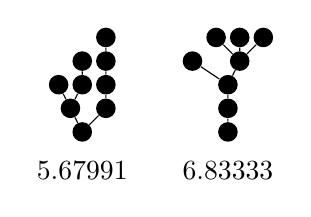
\begin{tikzpicture}[scale=.2, anchor=south]
      \node[circle, scale=0.75, fill] (tid1) at (2.25,3){};
      \node[circle, scale=0.75, fill] (tid3) at (1.5,4.5){};
      \node[circle, scale=0.75, fill] (tid6) at (0.75,6){};
      \node[circle, scale=0.75, fill] (tid7) at (2.25,6){};
      \node[circle, scale=0.75, fill] (tid10) at (2.25,7.5){};
      \draw[](tid7) -- (tid10);
      \draw[](tid3) -- (tid6);
      \draw[](tid3) -- (tid7);
      \node[circle, scale=0.75, fill] (tid4) at (3.75,4.5){};
      \node[circle, scale=0.75, fill] (tid8) at (3.75,6){};
      \node[circle, scale=0.75, fill] (tid11) at (3.75,7.5){};
      \node[circle, scale=0.75, fill] (tid14) at (3.75,9){};
      \draw[](tid11) -- (tid14);
      \draw[](tid8) -- (tid11);
      \draw[](tid4) -- (tid8);
      \draw[](tid1) -- (tid3);
      \draw[](tid1) -- (tid4);
      \node at (2.25, 0){5.67991};
      \begin{scope}[xshift=4cm]
        \node[circle, scale=0.75, fill] (tid2) at (7.5,3){};
        \node[circle, scale=0.75, fill] (tid5) at (7.5,4.5){};
        \node[circle, scale=0.75, fill] (tid9) at (7.5,6){};
        \node[circle, scale=0.75, fill] (tid12) at (5.25,7.5){};
        \node[circle, scale=0.75, fill] (tid13) at (8.25,7.5){};
        \node[circle, scale=0.75, fill] (tid15) at (6.75,9){};
        \node[circle, scale=0.75, fill] (tid16) at (8.25,9){};
        \node[circle, scale=0.75, fill] (tid17) at (9.75,9){};
        \draw[](tid13) -- (tid15);
        \draw[](tid13) -- (tid16);
        \draw[](tid13) -- (tid17);
        \draw[](tid9) -- (tid12);
        \draw[](tid9) -- (tid13);
        \draw[](tid5) -- (tid9);
        \draw[](tid2) -- (tid5);
        \node at (7.5, 0){6.83333};
      \end{scope}
    \end{tikzpicture}  
    \caption{Removing the root yields two subtrees with optimal expected runtimes (for three processors) as noted.}
  \end{subfigure}
  \caption{Intree $(0,0,1,1,2,3,3,4,5,7,8,9,9,11,13,13,13)$ and its corresponding subtrees rooted at the root's predecessors}
  \label{fig:reasoning-for-longest-root-subtree}
\end{figure}

Once again, this strategy can be shown to be suboptimal by considering $(0,0,0,1,1,1,2,2,3)$ (as depicted in figure \ref{fig:hlfnfc-is-not-optimal}) whose root has the following three predecessor intrees.

\begin{center}
  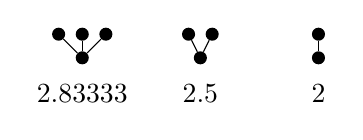
\begin{tikzpicture}[scale=.3]
    \begin{scope}
      \node[circle, fill, scale=.5] (0) at (0,0){};
      \node[circle, fill, scale=.5] (1) at (-1,1){};
      \node[circle, fill, scale=.5] (2) at (0,1){};
      \node[circle, fill, scale=.5] (3) at (1,1){};
      \draw(0)--(1);
      \draw(0)--(2);
      \draw(0)--(3);
      \node at (0, -1.5){2.83333};
    \end{scope}
    \begin{scope}[xshift=5cm]
      \node[circle, fill, scale=.5] (0) at (0,0){};
      \node[circle, fill, scale=.5] (1) at (-.5,1){};
      \node[circle, fill, scale=.5] (3) at (.5,1){};
      \draw(0)--(1);
      \draw(0)--(3);
      \node at (0, -1.5){2.5};
    \end{scope}
    \begin{scope}[xshift=10cm]
      \node[circle, fill, scale=.5] (0) at (0,0){};
      \node[circle, fill, scale=.5] (1) at (0,1){};
      \draw(0)--(1);
      \node at (0, -1.5){2};
    \end{scope}
  \end{tikzpicture}
\end{center}

For the intree $(0,0,0,1,1,1,2,2,3)$ the optimal schedule initially chooses the tasks 7,8 and 9 (the respective subtrees have run times 2.5 and 2).

\emph{Remark:} This intree \emph{might} not be the minimal intree serving as a counter example. Still, it is small and simple enough to be easily comprehensible.

\subsection{Preferring root's predecessors with shortest processing time}
\label{sec:suboptimal-preferring-root-predecessors-shortest-time}

It is clear that the opposite of the strategy from section \ref{sec:suboptimal-hlf-can-roots-longest-predecessors}, namely preferring those subtrees whose processing time is shortest, does also not yield correct results. This can be easily seen by considering the intree $(0,1,2,3,0,5,6,0,8,0)$ that is optimally scheduled by HLF (see section \ref{sec:p3-parallel-chains} for a proof) and whose root has the three following predecessors:

\begin{center}
  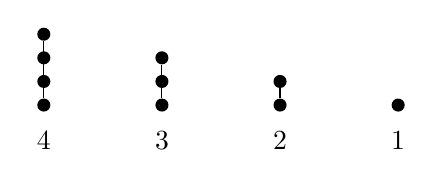
\begin{tikzpicture}[scale=.3]
    \begin{scope}[xshift=15cm]
      \node[circle, fill, scale=.5] (0) at (0,0){};
      \node[circle, fill, scale=.5] (1) at (0,1){};
      \node[circle, fill, scale=.5] (2) at (0,2){};
      \node[circle, fill, scale=.5] (3) at (0,3){};
      \draw(0)--(3);
      \node at (0, -1.5){4};
    \end{scope}
    \begin{scope}[xshift=20cm]
      \node[circle, fill, scale=.5] (0) at (0,0){};
      \node[circle, fill, scale=.5] (1) at (0,1){};
      \node[circle, fill, scale=.5] (2) at (0,2){};
      \draw(0)--(2);
      \node at (0, -1.5){3};
    \end{scope}
    \begin{scope}[xshift=25cm]
      \node[circle, fill, scale=.5] (0) at (0,0){};
      \node[circle, fill, scale=.5] (1) at (0,1){};
      \draw(0)--(1);
      \node at (0, -1.5){2};
    \end{scope}
    \begin{scope}[xshift=30cm]
      \node[circle, fill, scale=.5] (0) at (0,0){};
      \draw(0)--(0);
      \node at (0, -1.5){1};
    \end{scope}
  \end{tikzpicture}
\end{center}

\subsection{``Filling up subtrees''}
\label{sec:suboptimal-filling-subtrees}

We observed that (for three processors) an optimal schedule looks as if it chose certain subtrees and ``filled them up one after another''. This is probably most concise formalized as the following pattern:

\begin{itemize}
\item Identify disjoint leaf-maximal (or topmost-maximal) subtrees of the whole intree.
\item Assign priorities to the subtrees so they are sorted according to this priority (thus, we have a sequence of subtrees $S_1,\dots,S_r$).
\item Schedule as many tasks from $S_1$ as possible. If all ready tasks in $S_1$ are scheduled, schedule as many tasks as possible in $S_2$. If all tasks in $S_2$ are scheduled, schedule as many tasks as possible in $S_3$.
\end{itemize}

The main suspicion for this strategy was that an optimal schedule -- in the beginning -- does not ``switch'' to the next subtree if the current subtree has more unscheduled topmost tasks.

%In an optimal schedule, we can -- without loss of generality -- assume that it is \emph{not} the case that there are two distinct scheduled tasks $x$ and $y$ with different successors and each of them having a non-scheduled, but ready task.

An alternative formulation of the above strategy states that there is at most one task having both scheduled and non-scheduled predecessors that are leaves. 

It can be easily seen that there are optimal schedules violating this property, e.g. for the intree $(0,0,0,1,1,2,2,3)$. But for this intree (and \emph{many} others for whith optimal schedules violate this property), there is another schedule having \emph{exact the same} run time but fulfilling the property.

The example intree $(0,0,0,1,1,2,2,3)$ admits two different schedules (one beginning with tasks 4,5,8 and the other beginning with 4,6,8) that have exactly the same run time (see figure \ref{fig:filling-up-without-loss-of-generality}). The reason is that both schedules result in equivalent snapshots with the same probabilities after the first task finishes.

\begin{figure}[th]
  \centering
  \begin{subfigure}{.45\textwidth}
    \centering
    \renewcommand{\leveltopI}{-15cm + \leveltop}
\renewcommand{\leveltopII}{-15cm + \leveltopI}
\renewcommand{\leveltopIII}{-15cm + \leveltopII}
\renewcommand{\leveltopIIII}{-15cm + \leveltopIII}
\renewcommand{\leveltopIIIII}{-15cm + \leveltopIIII}
\renewcommand{\leveltopIIIIII}{-15cm + \leveltopIIIII}
\renewcommand{\leveltopIIIIIII}{-15cm + \leveltopIIIIII}
\renewcommand{\leveltopIIIIIIII}{-15cm + \leveltopIIIIIII}
\renewcommand{\leveltopIIIIIIIII}{-15cm + \leveltopIIIIIIII}
\begin{tikzpicture}[scale=.2, anchor=south]
\begin{scope}[yshift=\leveltopI cm]
\matrix (line1)[column sep=1cm] {
\node[draw=black, rectangle split,  rectangle split parts=4] (sn0x9a15218){
\footnotesize{100}
\nodepart{two}
\begin{tikzpicture}[scale=.2]
\node[circle, scale=0.75, fill] (tid0) at (3.75,1.5){};
\node[circle, scale=0.75, fill] (tid1) at (1.5,3){};
\node[circle, scale=0.75, fill, task_scheduled] (tid4) at (0.75,4.5){};
\node[circle, scale=0.75, fill, task_scheduled] (tid5) at (2.25,4.5){};
\draw[](tid1) -- (tid4);
\draw[](tid1) -- (tid5);
\node[circle, scale=0.75, fill] (tid2) at (3.75,3){};
\node[circle, scale=0.75, fill, task_scheduled] (tid6) at (3.75,4.5){};
\draw[](tid2) -- (tid6);
\node[circle, scale=0.75, fill] (tid3) at (6,3){};
\node[circle, scale=0.75, fill] (tid7) at (5.25,4.5){};
\node[circle, scale=0.75, fill] (tid8) at (6.75,4.5){};
\draw[](tid3) -- (tid7);
\draw[](tid3) -- (tid8);
\draw[](tid0) -- (tid1);
\draw[](tid0) -- (tid2);
\draw[](tid0) -- (tid3);
\end{tikzpicture}
\nodepart{three}
\footnotesize{4.87243}
\nodepart{four}
\footnotesize{$33\:67$}
};
 & 
\\
};
\end{scope}
\begin{scope}[yshift=\leveltopII cm]
\matrix (line2)[column sep=1cm] {
\node[draw=black, rectangle split,  rectangle split parts=4] (sn0x9a15160){
\footnotesize{33.3333}
\nodepart{two}
\begin{tikzpicture}[scale=.2]
\node[circle, scale=0.75, fill] (tid0) at (3.75,1.5){};
\node[circle, scale=0.75, fill] (tid1) at (0.75,3){};
\node[circle, scale=0.75, fill] (tid2) at (3,3){};
\node[circle, scale=0.75, fill, task_scheduled] (tid4) at (2.25,4.5){};
\node[circle, scale=0.75, fill, task_scheduled] (tid5) at (3.75,4.5){};
\draw[](tid2) -- (tid4);
\draw[](tid2) -- (tid5);
\node[circle, scale=0.75, fill] (tid3) at (6,3){};
\node[circle, scale=0.75, fill, task_scheduled] (tid6) at (5.25,4.5){};
\node[circle, scale=0.75, fill] (tid7) at (6.75,4.5){};
\draw[](tid3) -- (tid6);
\draw[](tid3) -- (tid7);
\draw[](tid0) -- (tid1);
\draw[](tid0) -- (tid2);
\draw[](tid0) -- (tid3);
\end{tikzpicture}
\nodepart{three}
\footnotesize{4.53704}
\nodepart{four}
\footnotesize{$1$}
};
 & 
\node[draw=black, rectangle split,  rectangle split parts=4] (sn0x9a14bc0){
\footnotesize{66.6667}
\nodepart{two}
\begin{tikzpicture}[scale=.2]
\node[circle, scale=0.75, fill] (tid0) at (3,1.5){};
\node[circle, scale=0.75, fill] (tid1) at (1.5,3){};
\node[circle, scale=0.75, fill, task_scheduled] (tid4) at (0.75,4.5){};
\node[circle, scale=0.75, fill] (tid5) at (2.25,4.5){};
\draw[](tid1) -- (tid4);
\draw[](tid1) -- (tid5);
\node[circle, scale=0.75, fill] (tid2) at (3.75,3){};
\node[circle, scale=0.75, fill, task_scheduled] (tid6) at (3.75,4.5){};
\draw[](tid2) -- (tid6);
\node[circle, scale=0.75, fill] (tid3) at (5.25,3){};
\node[circle, scale=0.75, fill, task_scheduled] (tid7) at (5.25,4.5){};
\draw[](tid3) -- (tid7);
\draw[](tid0) -- (tid1);
\draw[](tid0) -- (tid2);
\draw[](tid0) -- (tid3);
\end{tikzpicture}
\nodepart{three}
\footnotesize{4.54012}
\nodepart{four}
\footnotesize{$67\:33$}
};
 & 
\\
};
\end{scope}
\draw (sn0x9a15218.south) -- (sn0x9a14bc0.north);
\draw (sn0x9a15218.south) -- (sn0x9a15160.north);
\end{tikzpicture}
%%% Local Variables:
%%% TeX-master: "thesis/thesis.tex"
%%% End: 

    \caption{Optimal schedule starting with tasks 4,5 and 8.}
  \end{subfigure}
  \quad
  \begin{subfigure}{.45\textwidth}
    \centering
    \renewcommand{\leveltopI}{-15cm + \leveltop}
\renewcommand{\leveltopII}{-15cm + \leveltopI}
\renewcommand{\leveltopIII}{-15cm + \leveltopII}
\renewcommand{\leveltopIIII}{-15cm + \leveltopIII}
\renewcommand{\leveltopIIIII}{-15cm + \leveltopIIII}
\renewcommand{\leveltopIIIIII}{-15cm + \leveltopIIIII}
\renewcommand{\leveltopIIIIIII}{-15cm + \leveltopIIIIII}
\renewcommand{\leveltopIIIIIIII}{-15cm + \leveltopIIIIIII}
\renewcommand{\leveltopIIIIIIIII}{-15cm + \leveltopIIIIIIII}
\begin{tikzpicture}[scale=.2, anchor=south]
\begin{scope}[yshift=\leveltopI cm]
\matrix (line1)[column sep=1cm] {
\node[draw=black, rectangle split,  rectangle split parts=4] (sn0x91bd598){
\footnotesize{100}
\nodepart{two}
\begin{tikzpicture}[scale=.2]
\node[circle, scale=0.75, fill] (tid0) at (3.75,1.5){};
\node[circle, scale=0.75, fill] (tid1) at (1.5,3){};
\node[circle, scale=0.75, fill, task_scheduled] (tid4) at (0.75,4.5){};
\node[circle, scale=0.75, fill] (tid5) at (2.25,4.5){};
\draw[](tid1) -- (tid4);
\draw[](tid1) -- (tid5);
\node[circle, scale=0.75, fill] (tid2) at (4.5,3){};
\node[circle, scale=0.75, fill, task_scheduled] (tid6) at (3.75,4.5){};
\node[circle, scale=0.75, fill] (tid7) at (5.25,4.5){};
\draw[](tid2) -- (tid6);
\draw[](tid2) -- (tid7);
\node[circle, scale=0.75, fill] (tid3) at (6.75,3){};
\node[circle, scale=0.75, fill, task_scheduled] (tid8) at (6.75,4.5){};
\draw[](tid3) -- (tid8);
\draw[](tid0) -- (tid1);
\draw[](tid0) -- (tid2);
\draw[](tid0) -- (tid3);
\end{tikzpicture}
\nodepart{three}
\footnotesize{4.87243}
\nodepart{four}
\footnotesize{$33\:67$}
};
 & 
\\
};
\end{scope}
\begin{scope}[yshift=\leveltopII cm]
\matrix (line2)[column sep=1cm] {
\node[draw=black, rectangle split,  rectangle split parts=4] (sn0x91bd160){
\footnotesize{33.3333}
\nodepart{two}
\begin{tikzpicture}[scale=.2]
\node[circle, scale=0.75, fill] (tid0) at (3.75,1.5){};
\node[circle, scale=0.75, fill] (tid1) at (0.75,3){};
\node[circle, scale=0.75, fill] (tid2) at (3,3){};
\node[circle, scale=0.75, fill, task_scheduled] (tid4) at (2.25,4.5){};
\node[circle, scale=0.75, fill, task_scheduled] (tid5) at (3.75,4.5){};
\draw[](tid2) -- (tid4);
\draw[](tid2) -- (tid5);
\node[circle, scale=0.75, fill] (tid3) at (6,3){};
\node[circle, scale=0.75, fill, task_scheduled] (tid6) at (5.25,4.5){};
\node[circle, scale=0.75, fill] (tid7) at (6.75,4.5){};
\draw[](tid3) -- (tid6);
\draw[](tid3) -- (tid7);
\draw[](tid0) -- (tid1);
\draw[](tid0) -- (tid2);
\draw[](tid0) -- (tid3);
\end{tikzpicture}
\nodepart{three}
\footnotesize{4.53704}
\nodepart{four}
\footnotesize{$1$}
};
 & 
\node[draw=black, rectangle split,  rectangle split parts=4] (sn0x91bcbc0){
\footnotesize{66.6667}
\nodepart{two}
\begin{tikzpicture}[scale=.2]
\node[circle, scale=0.75, fill] (tid0) at (3,1.5){};
\node[circle, scale=0.75, fill] (tid1) at (1.5,3){};
\node[circle, scale=0.75, fill, task_scheduled] (tid4) at (0.75,4.5){};
\node[circle, scale=0.75, fill] (tid5) at (2.25,4.5){};
\draw[](tid1) -- (tid4);
\draw[](tid1) -- (tid5);
\node[circle, scale=0.75, fill] (tid2) at (3.75,3){};
\node[circle, scale=0.75, fill, task_scheduled] (tid6) at (3.75,4.5){};
\draw[](tid2) -- (tid6);
\node[circle, scale=0.75, fill] (tid3) at (5.25,3){};
\node[circle, scale=0.75, fill, task_scheduled] (tid7) at (5.25,4.5){};
\draw[](tid3) -- (tid7);
\draw[](tid0) -- (tid1);
\draw[](tid0) -- (tid2);
\draw[](tid0) -- (tid3);
\end{tikzpicture}
\nodepart{three}
\footnotesize{4.54012}
\nodepart{four}
\footnotesize{$67\:33$}
};
 & 
\\
};
\end{scope}
\draw (sn0x91bd598.south) -- (sn0x91bcbc0.north);
\draw (sn0x91bd598.south) -- (sn0x91bd160.north);
\end{tikzpicture}
%%% Local Variables:
%%% TeX-master: "thesis/thesis.tex"
%%% End: 

    \caption{Optimal schedule starting with tasks 4,6 and 8.}
  \end{subfigure}
  \caption{The intree $(0,0,0,1,1,2,2,3)$ has two different schedules reaching the optimum expected run time.}
  \label{fig:filling-up-without-loss-of-generality}
\end{figure}

For trees with fewer than 12 tasks, we could not find any tree that violated our conjecture in the sense that there would be \emph{only one single optimal schedule} violating it. However, the intree $(0,0,0,2,2,3,5,5,6,6,6)$ has the interesting property that the optimal schedule for this intree has to schedule tasks such that the intree contains two tasks that have as well scheduled as non-scheduled but ready predecessors. Figure \ref{fig:filling-op-is-not-strictly-optimal} shows the first steps of an optimal schedule for this intree.

\begin{figure}[th]
  \centering
  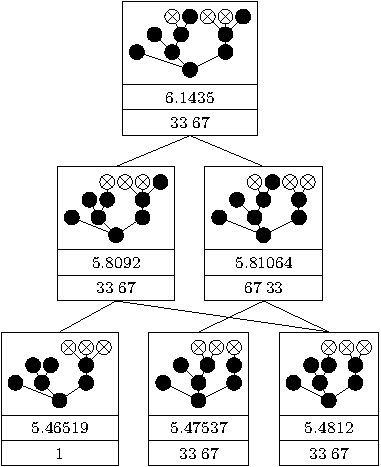
\includegraphics{p3/suboptimal/00022355666_optimal_no_fill_up.pdf}
  \caption{The optimal schedule for $(0,0,0,2,2,3,5,5,6,6,6)$ has two tasks (5 and 6) that have both scheduled and non-scheduled leaves as predecessors.}
  \label{fig:filling-op-is-not-strictly-optimal}
\end{figure}

\emph{Remark:} Surprisingly, every subtree of $(0,0,0,2,2,3,5,5,6,6,6)$ fulfills the conjecture that there is at most one task that has both scheduled and non-scheduled leaves as predecessors (during the whole schedule). This shows that even tasks that \emph{might seem} of minor impact (such as e.g. task 1 in the intree) for the first choices, might be relevant to the question which tasks are chosen in the optimal schedule.

\subsection{As many topmost tasks as possible}
\label{sec:suboptimal-hlf-refinement-as-many-topmost-possible}

During our research, we recognized that in many cases, the optimal schedule consists only of snapshots where \emph{as many topmost tasks} as possible are scheduled. This is true for all intrees with up to 12 tasks.

However, there is an optimal schedule for an intree with 13 tasks that violates this condition ---  the intree $(0,0,1,2,3,4,5,5,5,7,10,11)$ (shown in figure \ref{fig:as-many-topmost-tasks-as-possible-false}). This intree comes into a situation where it has -- \emph{due to previous choices} -- three topmost tasks, of which only two are scheduled.

\begin{figure}[th]
  \centering
  \renewcommand{\leveltopI}{-18cm + \leveltop}
\renewcommand{\leveltopII}{-18cm + \leveltopI}
\renewcommand{\leveltopIII}{-18cm + \leveltopII}
\renewcommand{\leveltopIIII}{-18cm + \leveltopIII}
\renewcommand{\leveltopIIIII}{-18cm + \leveltopIIII}
\renewcommand{\leveltopIIIIII}{-18cm + \leveltopIIIII}
\renewcommand{\leveltopIIIIIII}{-18cm + \leveltopIIIIII}
\renewcommand{\leveltopIIIIIIII}{-18cm + \leveltopIIIIIII}
\renewcommand{\leveltopIIIIIIIII}{-18cm + \leveltopIIIIIIII}
\renewcommand{\leveltopIIIIIIIIII}{-18cm + \leveltopIIIIIIIII}
\renewcommand{\leveltopIIIIIIIIIII}{-18cm + \leveltopIIIIIIIIII}
\renewcommand{\leveltopIIIIIIIIIIII}{-18cm + \leveltopIIIIIIIIIII}
\renewcommand{\leveltopIIIIIIIIIIIII}{-18cm + \leveltopIIIIIIIIIIII}
\begin{tikzpicture}[scale=.2, anchor=south]
\begin{scope}[yshift=\leveltopI cm]
\matrix (line1)[column sep=0.5cm] {
\node[draw=black, rectangle split,  rectangle split parts=3] (sn0x96804c8){
\begin{tikzpicture}[scale=.2]
\node[circle, scale=0.75, fill] (tid0) at (3,1.5){};
\node[circle, scale=0.75, fill] (tid1) at (0.75,3){};
\node[circle, scale=0.75, fill] (tid3) at (0.75,4.5){};
\node[circle, scale=0.75, fill, task_scheduled] (tid5) at (0.75,6){};
\draw[](tid3) -- (tid5);
\draw[](tid1) -- (tid3);
\node[circle, scale=0.75, fill] (tid2) at (3.75,3){};
\node[circle, scale=0.75, fill] (tid4) at (3.75,4.5){};
\node[circle, scale=0.75, fill] (tid6) at (3.75,6){};
\node[circle, scale=0.75, fill, task_scheduled] (tid7) at (2.25,7.5){};
\node[circle, scale=0.75, fill] (tid8) at (3.75,7.5){};
\node[circle, scale=0.75, fill] (tid9) at (5.25,7.5){};
\node[circle, scale=0.75, fill] (tid10) at (5.25,9){};
\node[circle, scale=0.75, fill] (tid11) at (5.25,10.5){};
\node[circle, scale=0.75, fill, task_scheduled] (tid12) at (5.25,12){};
\draw[](tid11) -- (tid12);
\draw[](tid10) -- (tid11);
\draw[](tid9) -- (tid10);
\draw[](tid6) -- (tid7);
\draw[](tid6) -- (tid8);
\draw[](tid6) -- (tid9);
\draw[](tid4) -- (tid6);
\draw[](tid2) -- (tid4);
\draw[](tid0) -- (tid1);
\draw[](tid0) -- (tid2);
\end{tikzpicture}
\nodepart{two}
\footnotesize{8.28398}
\nodepart{three}
\footnotesize{$33\:33\:33$}
};
 & 
\\
};
\end{scope}
\begin{scope}[yshift=\leveltopII cm]
\matrix (line2)[column sep=0.5cm] {
\node[draw=black, rectangle split,  rectangle split parts=3] (sn0x9680470){
\begin{tikzpicture}[scale=.2]
\node[circle, scale=0.75, fill] (tid0) at (3,1.5){};
\node[circle, scale=0.75, fill] (tid1) at (0.75,3){};
\node[circle, scale=0.75, fill] (tid3) at (0.75,4.5){};
\node[circle, scale=0.75, fill, task_scheduled] (tid5) at (0.75,6){};
\draw[](tid3) -- (tid5);
\draw[](tid1) -- (tid3);
\node[circle, scale=0.75, fill] (tid2) at (3.75,3){};
\node[circle, scale=0.75, fill] (tid4) at (3.75,4.5){};
\node[circle, scale=0.75, fill] (tid6) at (3.75,6){};
\node[circle, scale=0.75, fill, task_scheduled] (tid7) at (2.25,7.5){};
\node[circle, scale=0.75, fill] (tid8) at (3.75,7.5){};
\node[circle, scale=0.75, fill] (tid9) at (5.25,7.5){};
\node[circle, scale=0.75, fill] (tid10) at (5.25,9){};
\node[circle, scale=0.75, fill, task_scheduled] (tid11) at (5.25,10.5){};
\draw[](tid10) -- (tid11);
\draw[](tid9) -- (tid10);
\draw[](tid6) -- (tid7);
\draw[](tid6) -- (tid8);
\draw[](tid6) -- (tid9);
\draw[](tid4) -- (tid6);
\draw[](tid2) -- (tid4);
\draw[](tid0) -- (tid1);
\draw[](tid0) -- (tid2);
\end{tikzpicture}
\nodepart{two}
\footnotesize{7.48903}
\nodepart{three}
\footnotesize{$33\:33\:33$}
};
 & 
\node[draw=black, rectangle split,  rectangle split parts=3] (sn0x967eee0){
\begin{tikzpicture}[scale=.2]
\node[circle, scale=0.75, fill] (tid0) at (3,1.5){};
\node[circle, scale=0.75, fill] (tid1) at (0.75,3){};
\node[circle, scale=0.75, fill] (tid3) at (0.75,4.5){};
\draw[](tid1) -- (tid3);
\node[circle, scale=0.75, fill] (tid2) at (3.75,3){};
\node[circle, scale=0.75, fill] (tid4) at (3.75,4.5){};
\node[circle, scale=0.75, fill] (tid5) at (3.75,6){};
\node[circle, scale=0.75, fill, task_scheduled] (tid6) at (2.25,7.5){};
\node[circle, scale=0.75, fill, task_scheduled] (tid7) at (3.75,7.5){};
\node[circle, scale=0.75, fill] (tid8) at (5.25,7.5){};
\node[circle, scale=0.75, fill] (tid9) at (5.25,9){};
\node[circle, scale=0.75, fill] (tid10) at (5.25,10.5){};
\node[circle, scale=0.75, fill, task_scheduled] (tid11) at (5.25,12){};
\draw[](tid10) -- (tid11);
\draw[](tid9) -- (tid10);
\draw[](tid8) -- (tid9);
\draw[](tid5) -- (tid6);
\draw[](tid5) -- (tid7);
\draw[](tid5) -- (tid8);
\draw[](tid4) -- (tid5);
\draw[](tid2) -- (tid4);
\draw[](tid0) -- (tid1);
\draw[](tid0) -- (tid2);
\end{tikzpicture}
\nodepart{two}
\footnotesize{8.17577}
\nodepart{three}
\footnotesize{$33\:67$}
};
 & 
\node[draw=black, rectangle split,  rectangle split parts=3] (sn0x967f850){
\begin{tikzpicture}[scale=.2]
\node[circle, scale=0.75, fill] (tid0) at (2.25,1.5){};
\node[circle, scale=0.75, fill] (tid1) at (0.75,3){};
\node[circle, scale=0.75, fill] (tid3) at (0.75,4.5){};
\node[circle, scale=0.75, fill, task_scheduled] (tid5) at (0.75,6){};
\draw[](tid3) -- (tid5);
\draw[](tid1) -- (tid3);
\node[circle, scale=0.75, fill] (tid2) at (3,3){};
\node[circle, scale=0.75, fill] (tid4) at (3,4.5){};
\node[circle, scale=0.75, fill] (tid6) at (3,6){};
\node[circle, scale=0.75, fill, task_scheduled] (tid7) at (2.25,7.5){};
\node[circle, scale=0.75, fill] (tid8) at (3.75,7.5){};
\node[circle, scale=0.75, fill] (tid9) at (3.75,9){};
\node[circle, scale=0.75, fill] (tid10) at (3.75,10.5){};
\node[circle, scale=0.75, fill, task_scheduled] (tid11) at (3.75,12){};
\draw[](tid10) -- (tid11);
\draw[](tid9) -- (tid10);
\draw[](tid8) -- (tid9);
\draw[](tid6) -- (tid7);
\draw[](tid6) -- (tid8);
\draw[](tid4) -- (tid6);
\draw[](tid2) -- (tid4);
\draw[](tid0) -- (tid1);
\draw[](tid0) -- (tid2);
\end{tikzpicture}
\nodepart{two}
\footnotesize{8.18713}
\nodepart{three}
\footnotesize{$33\:33\:33$}
};
 & 
\\
};
\end{scope}
\begin{scope}[yshift=\leveltopIII cm]
\matrix (line3)[column sep=0.5cm] {
\node[draw=black, rectangle split,  rectangle split parts=3] (sn0x9680380){
\begin{tikzpicture}[scale=.2]
\node[circle, scale=0.75, fill] (tid0) at (3,1.5){};
\node[circle, scale=0.75, fill] (tid1) at (0.75,3){};
\node[circle, scale=0.75, fill] (tid3) at (0.75,4.5){};
\node[circle, scale=0.75, fill, task_scheduled] (tid5) at (0.75,6){};
\draw[](tid3) -- (tid5);
\draw[](tid1) -- (tid3);
\node[circle, scale=0.75, fill] (tid2) at (3.75,3){};
\node[circle, scale=0.75, fill] (tid4) at (3.75,4.5){};
\node[circle, scale=0.75, fill] (tid6) at (3.75,6){};
\node[circle, scale=0.75, fill, task_scheduled] (tid7) at (2.25,7.5){};
\node[circle, scale=0.75, fill] (tid8) at (3.75,7.5){};
\node[circle, scale=0.75, fill] (tid9) at (5.25,7.5){};
\node[circle, scale=0.75, fill, task_scheduled] (tid10) at (5.25,9){};
\draw[](tid9) -- (tid10);
\draw[](tid6) -- (tid7);
\draw[](tid6) -- (tid8);
\draw[](tid6) -- (tid9);
\draw[](tid4) -- (tid6);
\draw[](tid2) -- (tid4);
\draw[](tid0) -- (tid1);
\draw[](tid0) -- (tid2);
\end{tikzpicture}
\nodepart{two}
\footnotesize{6.81761}
\nodepart{three}
\footnotesize{$33\:33\:33$}
};
 & 
\node[draw=black, rectangle split,  rectangle split parts=3] (sn0x967ee48){
\begin{tikzpicture}[scale=.2]
\node[circle, scale=0.75, fill] (tid0) at (3,1.5){};
\node[circle, scale=0.75, fill] (tid1) at (0.75,3){};
\node[circle, scale=0.75, fill] (tid3) at (0.75,4.5){};
\draw[](tid1) -- (tid3);
\node[circle, scale=0.75, fill] (tid2) at (3.75,3){};
\node[circle, scale=0.75, fill] (tid4) at (3.75,4.5){};
\node[circle, scale=0.75, fill] (tid5) at (3.75,6){};
\node[circle, scale=0.75, fill, task_scheduled] (tid6) at (2.25,7.5){};
\node[circle, scale=0.75, fill, task_scheduled] (tid7) at (3.75,7.5){};
\node[circle, scale=0.75, fill] (tid8) at (5.25,7.5){};
\node[circle, scale=0.75, fill] (tid9) at (5.25,9){};
\node[circle, scale=0.75, fill, task_scheduled] (tid10) at (5.25,10.5){};
\draw[](tid9) -- (tid10);
\draw[](tid8) -- (tid9);
\draw[](tid5) -- (tid6);
\draw[](tid5) -- (tid7);
\draw[](tid5) -- (tid8);
\draw[](tid4) -- (tid5);
\draw[](tid2) -- (tid4);
\draw[](tid0) -- (tid1);
\draw[](tid0) -- (tid2);
\end{tikzpicture}
\nodepart{two}
\footnotesize{7.32305}
\nodepart{three}
\footnotesize{$33\:67$}
};
 & 
\node[draw=black, rectangle split,  rectangle split parts=3] (sn0x967f730){
\begin{tikzpicture}[scale=.2]
\node[circle, scale=0.75, fill] (tid0) at (2.25,1.5){};
\node[circle, scale=0.75, fill] (tid1) at (0.75,3){};
\node[circle, scale=0.75, fill] (tid3) at (0.75,4.5){};
\node[circle, scale=0.75, fill, task_scheduled] (tid5) at (0.75,6){};
\draw[](tid3) -- (tid5);
\draw[](tid1) -- (tid3);
\node[circle, scale=0.75, fill] (tid2) at (3,3){};
\node[circle, scale=0.75, fill] (tid4) at (3,4.5){};
\node[circle, scale=0.75, fill] (tid6) at (3,6){};
\node[circle, scale=0.75, fill, task_scheduled] (tid7) at (2.25,7.5){};
\node[circle, scale=0.75, fill] (tid8) at (3.75,7.5){};
\node[circle, scale=0.75, fill] (tid9) at (3.75,9){};
\node[circle, scale=0.75, fill, task_scheduled] (tid10) at (3.75,10.5){};
\draw[](tid9) -- (tid10);
\draw[](tid8) -- (tid9);
\draw[](tid6) -- (tid7);
\draw[](tid6) -- (tid8);
\draw[](tid4) -- (tid6);
\draw[](tid2) -- (tid4);
\draw[](tid0) -- (tid1);
\draw[](tid0) -- (tid2);
\end{tikzpicture}
\nodepart{two}
\footnotesize{7.32644}
\nodepart{three}
\footnotesize{$33\:33\:33$}
};
 & 
\node[draw=black, rectangle split,  rectangle split parts=3] (sn0x967e6e8){
\begin{tikzpicture}[scale=.2]
\node[circle, scale=0.75, fill] (tid0) at (2.25,1.5){};
\node[circle, scale=0.75, fill] (tid1) at (0.75,3){};
\node[circle, scale=0.75, fill, task_scheduled] (tid3) at (0.75,4.5){};
\draw[](tid1) -- (tid3);
\node[circle, scale=0.75, fill] (tid2) at (3,3){};
\node[circle, scale=0.75, fill] (tid4) at (3,4.5){};
\node[circle, scale=0.75, fill] (tid5) at (3,6){};
\node[circle, scale=0.75, fill, task_scheduled] (tid6) at (2.25,7.5){};
\node[circle, scale=0.75, fill] (tid7) at (3.75,7.5){};
\node[circle, scale=0.75, fill] (tid8) at (3.75,9){};
\node[circle, scale=0.75, fill] (tid9) at (3.75,10.5){};
\node[circle, scale=0.75, fill, task_scheduled] (tid10) at (3.75,12){};
\draw[](tid9) -- (tid10);
\draw[](tid8) -- (tid9);
\draw[](tid7) -- (tid8);
\draw[](tid5) -- (tid6);
\draw[](tid5) -- (tid7);
\draw[](tid4) -- (tid5);
\draw[](tid2) -- (tid4);
\draw[](tid0) -- (tid1);
\draw[](tid0) -- (tid2);
\end{tikzpicture}
\nodepart{two}
\footnotesize{8.10213}
\nodepart{three}
\footnotesize{$33\:33\:33$}
};
 & 
\node[draw=black, rectangle split,  rectangle split parts=3] (sn0x967f4d0){
\begin{tikzpicture}[scale=.2]
\node[circle, scale=0.75, fill] (tid0) at (1.5,1.5){};
\node[circle, scale=0.75, fill] (tid1) at (0.75,3){};
\node[circle, scale=0.75, fill] (tid3) at (0.75,4.5){};
\node[circle, scale=0.75, fill, task_scheduled] (tid5) at (0.75,6){};
\draw[](tid3) -- (tid5);
\draw[](tid1) -- (tid3);
\node[circle, scale=0.75, fill] (tid2) at (2.25,3){};
\node[circle, scale=0.75, fill] (tid4) at (2.25,4.5){};
\node[circle, scale=0.75, fill] (tid6) at (2.25,6){};
\node[circle, scale=0.75, fill] (tid7) at (2.25,7.5){};
\node[circle, scale=0.75, fill] (tid8) at (2.25,9){};
\node[circle, scale=0.75, fill] (tid9) at (2.25,10.5){};
\node[circle, scale=0.75, fill, task_scheduled] (tid10) at (2.25,12){};
\draw[](tid9) -- (tid10);
\draw[](tid8) -- (tid9);
\draw[](tid7) -- (tid8);
\draw[](tid6) -- (tid7);
\draw[](tid4) -- (tid6);
\draw[](tid2) -- (tid4);
\draw[](tid0) -- (tid1);
\draw[](tid0) -- (tid2);
\end{tikzpicture}
\nodepart{two}
\footnotesize{8.13281}
\nodepart{three}
\footnotesize{$50\:50$}
};
 & 
\\
};
\end{scope}
\begin{scope}[yshift=\leveltopIIII cm]
\matrix (line4)[column sep=0.5cm] {
\node[draw=black, rectangle split,  rectangle split parts=3] (sn0x96802b0){
\begin{tikzpicture}[scale=.2]
\node[circle, scale=0.75, fill] (tid0) at (3,1.5){};
\node[circle, scale=0.75, fill] (tid1) at (0.75,3){};
\node[circle, scale=0.75, fill] (tid3) at (0.75,4.5){};
\node[circle, scale=0.75, fill, task_scheduled] (tid5) at (0.75,6){};
\draw[](tid3) -- (tid5);
\draw[](tid1) -- (tid3);
\node[circle, scale=0.75, fill] (tid2) at (3.75,3){};
\node[circle, scale=0.75, fill] (tid4) at (3.75,4.5){};
\node[circle, scale=0.75, fill] (tid6) at (3.75,6){};
\node[circle, scale=0.75, fill, task_scheduled] (tid7) at (2.25,7.5){};
\node[circle, scale=0.75, fill, task_scheduled] (tid8) at (3.75,7.5){};
\node[circle, scale=0.75, fill] (tid9) at (5.25,7.5){};
\draw[](tid6) -- (tid7);
\draw[](tid6) -- (tid8);
\draw[](tid6) -- (tid9);
\draw[](tid4) -- (tid6);
\draw[](tid2) -- (tid4);
\draw[](tid0) -- (tid1);
\draw[](tid0) -- (tid2);
\end{tikzpicture}
\nodepart{two}
\footnotesize{6.30864}
\nodepart{three}
\footnotesize{$67\:33$}
};
 & 
\node[draw=black, rectangle split,  rectangle split parts=3] (sn0x967f648){
\begin{tikzpicture}[scale=.2]
\node[circle, scale=0.75, fill] (tid0) at (2.25,1.5){};
\node[circle, scale=0.75, fill] (tid1) at (0.75,3){};
\node[circle, scale=0.75, fill] (tid3) at (0.75,4.5){};
\node[circle, scale=0.75, fill, task_scheduled] (tid5) at (0.75,6){};
\draw[](tid3) -- (tid5);
\draw[](tid1) -- (tid3);
\node[circle, scale=0.75, fill] (tid2) at (3,3){};
\node[circle, scale=0.75, fill] (tid4) at (3,4.5){};
\node[circle, scale=0.75, fill] (tid6) at (3,6){};
\node[circle, scale=0.75, fill, task_scheduled] (tid7) at (2.25,7.5){};
\node[circle, scale=0.75, fill] (tid8) at (3.75,7.5){};
\node[circle, scale=0.75, fill, task_scheduled] (tid9) at (3.75,9){};
\draw[](tid8) -- (tid9);
\draw[](tid6) -- (tid7);
\draw[](tid6) -- (tid8);
\draw[](tid4) -- (tid6);
\draw[](tid2) -- (tid4);
\draw[](tid0) -- (tid1);
\draw[](tid0) -- (tid2);
\end{tikzpicture}
\nodepart{two}
\footnotesize{6.56279}
\nodepart{three}
\footnotesize{$33\:33\:33$}
};
 & 
\node[draw=black, rectangle split,  rectangle split parts=3] (sn0x967ed40){
\begin{tikzpicture}[scale=.2]
\node[circle, scale=0.75, fill] (tid0) at (3,1.5){};
\node[circle, scale=0.75, fill] (tid1) at (0.75,3){};
\node[circle, scale=0.75, fill] (tid3) at (0.75,4.5){};
\draw[](tid1) -- (tid3);
\node[circle, scale=0.75, fill] (tid2) at (3.75,3){};
\node[circle, scale=0.75, fill] (tid4) at (3.75,4.5){};
\node[circle, scale=0.75, fill] (tid5) at (3.75,6){};
\node[circle, scale=0.75, fill, task_scheduled] (tid6) at (2.25,7.5){};
\node[circle, scale=0.75, fill, task_scheduled] (tid7) at (3.75,7.5){};
\node[circle, scale=0.75, fill] (tid8) at (5.25,7.5){};
\node[circle, scale=0.75, fill, task_scheduled] (tid9) at (5.25,9){};
\draw[](tid8) -- (tid9);
\draw[](tid5) -- (tid6);
\draw[](tid5) -- (tid7);
\draw[](tid5) -- (tid8);
\draw[](tid4) -- (tid5);
\draw[](tid2) -- (tid4);
\draw[](tid0) -- (tid1);
\draw[](tid0) -- (tid2);
\end{tikzpicture}
\nodepart{two}
\footnotesize{6.5814}
\nodepart{three}
\footnotesize{$33\:67$}
};
 & 
\node[draw=black, rectangle split,  rectangle split parts=3] (sn0x967e630){
\begin{tikzpicture}[scale=.2]
\node[circle, scale=0.75, fill] (tid0) at (2.25,1.5){};
\node[circle, scale=0.75, fill] (tid1) at (0.75,3){};
\node[circle, scale=0.75, fill, task_scheduled] (tid3) at (0.75,4.5){};
\draw[](tid1) -- (tid3);
\node[circle, scale=0.75, fill] (tid2) at (3,3){};
\node[circle, scale=0.75, fill] (tid4) at (3,4.5){};
\node[circle, scale=0.75, fill] (tid5) at (3,6){};
\node[circle, scale=0.75, fill, task_scheduled] (tid6) at (2.25,7.5){};
\node[circle, scale=0.75, fill] (tid7) at (3.75,7.5){};
\node[circle, scale=0.75, fill] (tid8) at (3.75,9){};
\node[circle, scale=0.75, fill, task_scheduled] (tid9) at (3.75,10.5){};
\draw[](tid8) -- (tid9);
\draw[](tid7) -- (tid8);
\draw[](tid5) -- (tid6);
\draw[](tid5) -- (tid7);
\draw[](tid4) -- (tid5);
\draw[](tid2) -- (tid4);
\draw[](tid0) -- (tid1);
\draw[](tid0) -- (tid2);
\end{tikzpicture}
\nodepart{two}
\footnotesize{7.19387}
\nodepart{three}
\footnotesize{$33\:33\:33$}
};
 & 
\node[draw=black, rectangle split,  rectangle split parts=3] (sn0x967f3f8){
\begin{tikzpicture}[scale=.2]
\node[circle, scale=0.75, fill] (tid0) at (1.5,1.5){};
\node[circle, scale=0.75, fill] (tid1) at (0.75,3){};
\node[circle, scale=0.75, fill] (tid3) at (0.75,4.5){};
\node[circle, scale=0.75, fill, task_scheduled] (tid5) at (0.75,6){};
\draw[](tid3) -- (tid5);
\draw[](tid1) -- (tid3);
\node[circle, scale=0.75, fill] (tid2) at (2.25,3){};
\node[circle, scale=0.75, fill] (tid4) at (2.25,4.5){};
\node[circle, scale=0.75, fill] (tid6) at (2.25,6){};
\node[circle, scale=0.75, fill] (tid7) at (2.25,7.5){};
\node[circle, scale=0.75, fill] (tid8) at (2.25,9){};
\node[circle, scale=0.75, fill, task_scheduled] (tid9) at (2.25,10.5){};
\draw[](tid8) -- (tid9);
\draw[](tid7) -- (tid8);
\draw[](tid6) -- (tid7);
\draw[](tid4) -- (tid6);
\draw[](tid2) -- (tid4);
\draw[](tid0) -- (tid1);
\draw[](tid0) -- (tid2);
\end{tikzpicture}
\nodepart{two}
\footnotesize{7.22266}
\nodepart{three}
\footnotesize{$50\:50$}
};
 & 
\node[draw=black, rectangle split,  rectangle split parts=3] (sn0x967e310){
\begin{tikzpicture}[scale=.2]
\node[circle, scale=0.75, fill] (tid0) at (1.5,1.5){};
\node[circle, scale=0.75, fill] (tid1) at (0.75,3){};
\node[circle, scale=0.75, fill, task_scheduled] (tid3) at (0.75,4.5){};
\draw[](tid1) -- (tid3);
\node[circle, scale=0.75, fill] (tid2) at (2.25,3){};
\node[circle, scale=0.75, fill] (tid4) at (2.25,4.5){};
\node[circle, scale=0.75, fill] (tid5) at (2.25,6){};
\node[circle, scale=0.75, fill] (tid6) at (2.25,7.5){};
\node[circle, scale=0.75, fill] (tid7) at (2.25,9){};
\node[circle, scale=0.75, fill] (tid8) at (2.25,10.5){};
\node[circle, scale=0.75, fill, task_scheduled] (tid9) at (2.25,12){};
\draw[](tid8) -- (tid9);
\draw[](tid7) -- (tid8);
\draw[](tid6) -- (tid7);
\draw[](tid5) -- (tid6);
\draw[](tid4) -- (tid5);
\draw[](tid2) -- (tid4);
\draw[](tid0) -- (tid1);
\draw[](tid0) -- (tid2);
\end{tikzpicture}
\nodepart{two}
\footnotesize{8.04297}
\nodepart{three}
\footnotesize{$50\:50$}
};
 & 
\node[draw=black, rectangle split,  rectangle split parts=3] (sn0x967d418){
\begin{tikzpicture}[scale=.2]
\node[circle, scale=0.75, fill] (tid0) at (2.25,1.5){};
\node[circle, scale=0.75, fill, task_scheduled] (tid1) at (0.75,3){};
\node[circle, scale=0.75, fill] (tid2) at (3,3){};
\node[circle, scale=0.75, fill] (tid3) at (3,4.5){};
\node[circle, scale=0.75, fill] (tid4) at (3,6){};
\node[circle, scale=0.75, fill, task_scheduled] (tid5) at (2.25,7.5){};
\node[circle, scale=0.75, fill] (tid6) at (3.75,7.5){};
\node[circle, scale=0.75, fill] (tid7) at (3.75,9){};
\node[circle, scale=0.75, fill] (tid8) at (3.75,10.5){};
\node[circle, scale=0.75, fill, task_scheduled] (tid9) at (3.75,12){};
\draw[](tid8) -- (tid9);
\draw[](tid7) -- (tid8);
\draw[](tid6) -- (tid7);
\draw[](tid4) -- (tid5);
\draw[](tid4) -- (tid6);
\draw[](tid3) -- (tid4);
\draw[](tid2) -- (tid3);
\draw[](tid0) -- (tid1);
\draw[](tid0) -- (tid2);
\end{tikzpicture}
\nodepart{two}
\footnotesize{8.06954}
\nodepart{three}
\footnotesize{$33\:33\:33$}
};
 & 
\\
};
\end{scope}
\draw (sn0x96804c8.south) -- (sn0x967eee0.north);
\draw (sn0x96804c8.south) -- (sn0x967f850.north);
\draw (sn0x96804c8.south) -- (sn0x9680470.north);
\draw (sn0x9680470.south) -- (sn0x967ee48.north);
\draw (sn0x9680470.south) -- (sn0x967f730.north);
\draw (sn0x9680470.south) -- (sn0x9680380.north);
\draw (sn0x967eee0.south) -- (sn0x967e6e8.north);
\draw (sn0x967eee0.south) -- (sn0x967ee48.north);
\draw (sn0x967f850.south) -- (sn0x967e6e8.north);
\draw (sn0x967f850.south) -- (sn0x967f4d0.north);
\draw (sn0x967f850.south) -- (sn0x967f730.north);
\draw (sn0x9680380.south) -- (sn0x967ed40.north);
\draw (sn0x9680380.south) -- (sn0x967f648.north);
\draw (sn0x9680380.south) -- (sn0x96802b0.north);
\draw (sn0x967ee48.south) -- (sn0x967e630.north);
\draw (sn0x967ee48.south) -- (sn0x967ed40.north);
\draw (sn0x967f730.south) -- (sn0x967e630.north);
\draw (sn0x967f730.south) -- (sn0x967f3f8.north);
\draw (sn0x967f730.south) -- (sn0x967f648.north);
\draw (sn0x967e6e8.south) -- (sn0x967d418.north);
\draw (sn0x967e6e8.south) -- (sn0x967e310.north);
\draw (sn0x967e6e8.south) -- (sn0x967e630.north);
\draw (sn0x967f4d0.south) -- (sn0x967e310.north);
\draw (sn0x967f4d0.south) -- (sn0x967f3f8.north);
\end{tikzpicture}
%%% Local Variables:
%%% TeX-master: "thesis/thesis.tex"
%%% End: 

  \caption{Optimal schedule for intree $(0,0,1,2,3,4,5,5,5,7,10,11)$: This intree is an example illustrating that an optimal schedule does not necessarily have as many topmost tasks as possible scheduled \emph{in each step}.}
  \label{fig:as-many-topmost-tasks-as-possible-false}
\end{figure}

\emph{Remark:} Even if it is not true that an optimal schedule has as many topmost tasks as possible scheduled \emph{in each step}, we did not find a single example whose \emph{initial} choice violated the conjecture that as many topmost tasks as possible should be scheduled. This is later summarized in conjecture \ref{conj:as-many-topmost-as-possibly}.

\section{Maximizing 3-processor-time, minimizing 1-processor time}
\label{sec:p3-disproving-long-p3-and-short-p1-time}

Up to now, we maily focused on the structure of the current intree to derive strategies --- which all turned out to be (not strictly, but still) suboptimal. We now inspect another, more involved approach.

If we have three processors in total, we can split the total run time into three parts: The time where all three processors are processing tasks, the time where one processor is idle and two are working, and the time where only one processor is working. For this section, we employ the following notation.

%We first define some variants of run time. We consider the overall run time and the time where -- within a schedule of an intree -- exactly $p$ processors are working (i.e. where exactly $p$ tasks are scheduled).

\begin{definition}[Run time and its variants]
  We denote by $T$ the expected run time for a schedule associated with an intree. 
  Moreover, we denote the expected time where exactly $p$ tasks are scheduled by $T_p$ (i.e. where exactly $p$ processors are busy).
\end{definition}

Note that $T$ actually describes an \emph{expected value}. Because of the linearity of expectation, we have that -- for three processors -- $T=T_1 + T_2 + T_3$. If we want to construct an optimal schedule for three processors, we might be tempted to think that (at least) one of the two following criteria should be fulfilled for the optimal schedule:

\begin{description}
\item[P3L] For the optimal schedule, $T_3$ should be maximal (over all schedules), i.e. we should exploit three processors as long as possible (in the expectation).
\item[P1S] For the optimal schedule, $T_1$ should be minimal (over all schedules), i.e. we should try to keep the expected time for which only one processor is working as short as possible.
\end{description}

Surprisingly, as we will see, \emph{both} of them are wrong (at least if considered separately).

\subsection{Comparing $T_1$, $T_2$ and $T_3$ for particular intrees}
\label{sec:comparing-t1-t2-t3-particular-intrees}

We compare the times where exactly one, two resp. three precessors are busy for selected intrees. We start by comparing the respective intrees that were investigated so far and whose optimal schedule is non-HLF. The results are shown in table \ref{tab:comparing-t1-t2-t3-selected-intrees}.

\begin{table}[th]
  \centering
  \begin{tabular}[ht]{l|ccc|ccc}
    \multirow{2}{*}{Intree} & \multicolumn{3}{c|}{(Suboptimal) HLF} & \multicolumn{3}{c}{Optimal schedule} \\
    & $T_3$ & $T_2$ & $T_1$ & $T_3^*$ & $T_2^*$ & $T_1^*$ \\
    \hline
    $(0,0,1,1,1,2)$ & 0.7778 & 1.0556 & 2.5556 & 0.8519 & 0.9259 & 2.5926 \\
    $(0,0,1,2,3,4,6,6,8,8)$ & 0.9630 & 2.1061 & 3.8989 & 1.1029 & 1.8267 & 4.0379 \\
    $(0,0,1,2,4,4,6,7,8,8)$ & 0.9698 & 1.4520 & 5.1865 & 1.0796 & 1.2329 & 5.2955 \\
    $(0,0,1,2,3,4,5,5,7,9,9)$ & 1.0288 & 2.1691 & 4.5754 & 1.1852 & 1.8628 & 4.7189 \\
    $(0,0,1,2,2,3,3,6,8,9,10,11,12)$ & 1.1231 & 1.7182 & 7.1942 & 1.2466 & 1.4713 & 7.3176 \\
    $(0,0,0,2,3,4,5,7,7,9,10,10)$ & 1.7905 & 1.6275 & 4.3736 & 1.8899 & 1.4323 & 4.4658 \\
    % the following needs some comment on "suboptimal hlf"
    $(0,0,0,1,1,1,2,2,3)$ & 2.0069 & 0.7843 & 2.4108 & 2.0137 & 0.7723 & 2.4143 \\ 
    $(0,0,1,1,2,3,3,4,5,7,8,9,9,11,(13)^3)$ 
      & 3.8694 & 1.6105 & 3.1709 & 3.8783 & 1.5927 & 3.1796 \\
    $(0, 0, 1, 2, 2, 2, 3, 3, 3, 4)$ & 1.9040 & 1.2574 & 2.7733 & 1.9095 & 1.2469 & 2.7778 \\
    $(0, 0, 1, 1, 1, 2, 5, 6, 6, 6, 6)$ & 2.2337 & 1.2643 & 2.7703 & 2.2428 & 1.2469 & 2.7778 \\
    $(0,0,0,2,2,3,5,5,6,6,6)$ & 2.4127 & 1.0310 & 2.7000 & 2.4171 & 1.0224 & 2.7040
  \end{tabular}
  \caption{Comparing times where exactly one, two resp. three processors are busy.}
  \label{tab:comparing-t1-t2-t3-selected-intrees}
\end{table}

We observe -- for the intrees considered here without exception -- that $T_3^* \geq T_3$ and (surprisingly) also $T_1^* \geq T_1$. As a consequence, we always have $T_2^* \leq T_2$. In the following, we will inspect some examples that show that this is not always the case.

\subsection{Maximizing $T_3$}
\label{sec:p3-disproving-long-p3}

We now show an intree proving that an optimal schedule does not necessarily maximize $T_3$, the time span where all three processors are busy.

Figure \ref{fig:p3-p3l-suboptimal-example} shows an example, where the optimal schedule keeps three processors busy for expected 0.77777 time steps, while a suboptimal schedule keeps three processors busy for a longer expected time, namely about 0.851852 time steps.

From this we can conclude that it may be advantageous in some cases to accept a shorter time with three busy processors, thereby possibly also decreasing the time where only one processor is busy and increasing the time where exactly two processors are busy.

\begin{figure}[ht]
  \centering
  \begin{subfigure}{.45\linewidth}
    \centering
    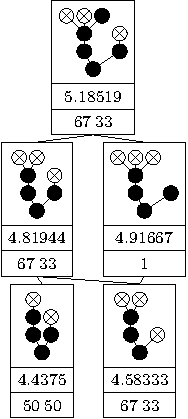
\includegraphics{p3/keep_3_busy/three_busy_subopt.pdf}
    \caption{This suboptimal schedule keeps three processors busy for expectedly $0.851852$ time steps ($(T_3, T_2, T_1)=(23/27,10/9,29/9)$).}
  \end{subfigure}
  \quad
  \begin{subfigure}{.45\linewidth}
    \centering
    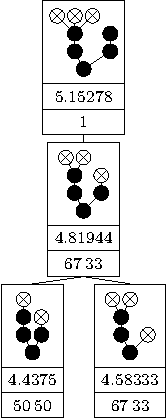
\includegraphics{p3/keep_3_busy/three_busy_opt.pdf}
    \caption{Optimal schedule. Keeps three processors busy for $7/9\approx 0.78$ time steps ($(T_3, T_2, T_1)=(7/9, 31/24, 37/12)$).}
  \end{subfigure}
  \caption{An intree that shows that an optimal P3 schedule needs not keep busy three processors as long as possible. Snapshots with fewer than 6 tasks omitted since they have at most two tasks to be scheduled can be (optimally) processed via ordinary HLF.}
  \label{fig:p3-p3l-suboptimal-example}
\end{figure}

\subsection{Minimizing $T_1$}
\label{sec:p3-disproving-short-p1}

The ``other direction'', i.e. minimizing the time with only one busy processor is suboptimal as well.
Figure \ref{fig:p3-p1s-suboptimal-example} shows an intree with the property that the optimal schedule has an expected timespan of roughly 2.59259, within which only one processor is busy. On the other hand, a suboptimal schedule has a timespan of roughly 2.55555 within which only one processor is busy.

\begin{figure}[ht]
  \centering
  \begin{subfigure}{.45\linewidth}
    \centering
    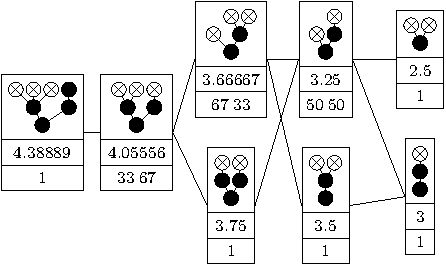
\includegraphics{p3/keep_1_unbusy/one_unbusy_subopt.pdf}
    \caption{This suboptimal schedule has an approximated timespan of $23/9\approx 2.55$, where only one processor is working ($(T_3, T_2, T_1)=(7/9,19/18,23/9)$).}
  \end{subfigure}
  \quad
  \begin{subfigure}{.45\linewidth}
    \centering
    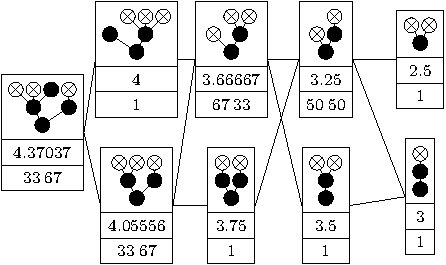
\includegraphics{p3/keep_1_unbusy/one_unbusy_opt.pdf}
    \caption{Optimal schedule. For expectedly $70/27\approx 2.59$ time steps, only one processor is busy $(T_3, T_2, T_1)=(23/27, 25/27, 70/27)$.}
  \end{subfigure}
  \caption{An intree where the expected time with only one processor being busy is longer within the optimal schedule ($\approx 2.59259$) than within a suboptimal schedule ($\approx 2.555555$).}
  \label{fig:p3-p1s-suboptimal-example}
\end{figure}

This shows that it can be useful to accept a longer time with only one processor busy, probably acchieving a longer time span where three processors are busy.

\subsection{Maximizing $T_3$ \emph{or} minimizing $T_1$}
\label{sec:p3-suboptimality-maximizing-t3-and-minimizing-t1}

It can also be shown that even combining the two arguments -- in the sense that P3L \emph{or} P1S should be fulfilled for the optimal schedule -- is not correct. This can be observed by examining the intree $(0, 0, 1, 1, 2, 3, 3, 3)$. Figure \ref{fig:p3l-p1s-combo-suboptimal} shows this example.

\begin{figure}[ht]
  \centering
  \begin{subfigure}{.3\linewidth}
    \centering
    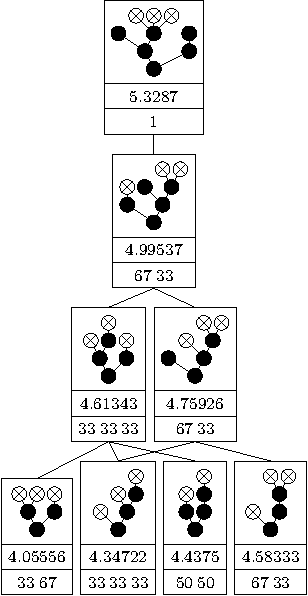
\includegraphics{p3/max_p3_min_p1/00112333opt.pdf}
    \caption{Optimal schedule. $(T_3^*,T_2^*,T_1^*)=(\frac{4}{3},\frac{217}{216},\frac{323}{108})$.}
  \end{subfigure}
  \quad
  \begin{subfigure}{.3\linewidth}
    \centering
    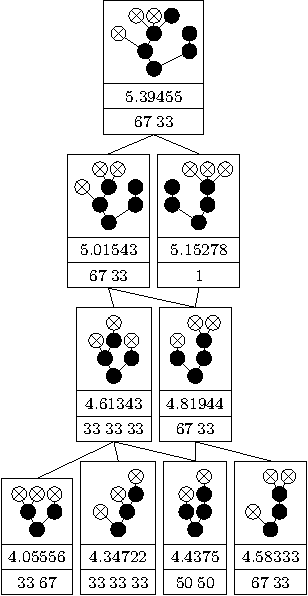
\includegraphics{p3/max_p3_min_p1/00112333t1min.pdf}
    \caption{Schedule with minimal $T_1$. $(T_3,T_2,T_1)=(\frac{290}{243},\frac{2369}{1944},\frac{2899}{972})$.}
  \end{subfigure}
  \quad
  \begin{subfigure}{.3\linewidth}
    \centering
    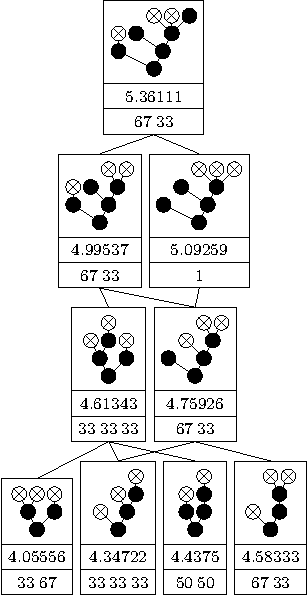
\includegraphics{p3/max_p3_min_p1/00112333t3max.pdf}
    \caption{Schedule with maximal $T_3$. $(T_3,T_2,T_1)=(\frac{110}{81},\frac{299}{324},\frac{499}{162})$.}
  \end{subfigure}
  \caption{A combination of P3L and P1S is not a criterion for an optimal schedule. The optimal schedule has $T_3^*=\frac{4}{3}\approx 1.333$ and $T_1^*=\frac{323}{108}\approx 2.99074$. One other (suboptimal) schedule has $T_1=\frac{2899}{972}\approx 2.98251 < T_1^*$, while still another schedule has $T_3=\frac{110}{81}\approx1.358025 > T_3^*$.}
  \label{fig:p3l-p1s-combo-suboptimal}
\end{figure}

\begin{corollary}
  Let $T^s$ denote the overall run time of a schedule $s$ and $T_1^s$, $T_2^s$ and $T_3^s$ be the times where exactly three, two and one tasks are scheduled within this schedule, respectively.

  Let $I$ be an intree and $S$ be the set of all schedules. Let $s^*$ be the optimal schedule, which has associated the optimal run time $T^*$, with $T_1^*, T_2^*, T_3^*$ being its parts.
  \begin{itemize}
  \item It may be the case that there is a schedule $s\in S$ such that $T_3^s \geq T_3^*$.
  \item It may be the case that there is a schedule $s\in S$ such that $T_1^s \leq T_1^*$.
  \end{itemize}
\end{corollary}

That is, it is not necessarily the case that $T_3$ is maximal for the optimal schedule, nor is it necessarily the case that $T_1$ is minimal for the optimal schedule.

However, after some investigation, we are tempted to conjecture the following.

\begin{conjecture}
  Let $I$, $T^s, T_1^s, T_2^s, T_3^s$ and $S$ be as defined above. Let $s^*$ be the optimal schedule for $I$ associated with the respective times $T_1^*, T_2^*, T_3^*$. Then, there is no schedule $s\in S$ such that
  \begin{equation*}
    T^s > T^* \wedge T_1^s \leq T_1^* \wedge T_3^s \geq T_3^*.
  \end{equation*}
\end{conjecture}

Even if this conjecture turned out to be true, it seems complex to transform this knowledge into a scheduling strategy that does something more significantly efficient than ``explore everything, and choose the best'' (i.e. LEAF scheduling with subsequent optimization), because $T_3, T_2$ and $T_1$ are not that easy to compute.

\paragraph{A note on implementation}
\label{sec:maximizing-t3-minimizing-t1-float-problem}

When we conducted experiments to find out whether $T_3$ must be maximal or $T_1$ must be minimal, we experienced the phenomenon that a floating point representation for expected values is not accurate enough for some measurements. This was one of the cases where we needed a representation by fractions (see sections \ref{sec:implementation-numbers} and \ref{sec:benchmarks-myfloat-variations}).

\section{Conclusion}
\label{sec:p3-conclusion}

Unfortunately, we did not find any strategy that always yields an optimal schedule. Of course, it is still possible to compute the optimal schedule by an exhaustive search.

During our research, we recognized some patterns that we are tempted to transform into conjectures. We were, however, not yet able to prove or disprove them. These conjectures might be used to reduce the number of snapshots that need to be examined by an exhaustive search used to compute the optimal snapshot.

This section sums up the most important conjectures we found.

\begin{conjecture}
  \label{conj:as-many-topmost-as-possibly}
  An optimal schedule initially schedules as many topmost tasks as possible. 
  In intermediate steps, if possible, it chooses a topmost task as the next task to be scheduled.
\end{conjecture}

Please note that the above conjecture does not state anything about \emph{which} topmost tasks should be chosen in order to generate a schedule that is as good as possible. It can -- however -- drastically reduce the number of choices for the tasks to be scheduled. As an example, consider the following tree:

\begin{center}
  \begin{tikzpicture}[scale=.2]
    \node[circle, scale=0.75, fill] (tid0) at (7.5,1.5){};
    \node[circle, scale=0.75, fill] (tid1) at (0.75,3){};
    \node[circle, scale=0.75, fill] (tid2) at (5.25,3){};
    \node[circle, scale=0.75, fill] (tid4) at (2.25,4.5){};
    \node[circle, scale=0.75, fill] (tid5) at (3.75,4.5){};
    \node[circle, scale=0.75, fill] (tid8) at (3.75,6){};
    \draw[](tid5) -- (tid8);
    \node[circle, scale=0.75, fill] (tid6) at (6.75,4.5){};
    \node[circle, scale=0.75, fill] (tid9) at (6,6){};
    \node[circle, scale=0.75, fill] (tid13) at (5.25,7.5){};
    \node[circle, scale=0.75, fill] (tid14) at (6.75,7.5){};
    \draw[](tid9) -- (tid13);
    \draw[](tid9) -- (tid14);
    \node[circle, scale=0.75, fill] (tid10) at (8.25,6){};
    \node[circle, scale=0.75, fill] (tid15) at (8.25,7.5){};
    \draw[](tid10) -- (tid15);
    \draw[](tid6) -- (tid9);
    \draw[](tid6) -- (tid10);
    \draw[](tid2) -- (tid4);
    \draw[](tid2) -- (tid5);
    \draw[](tid2) -- (tid6);
    \node[circle, scale=0.75, fill] (tid3) at (12,3){};
    \node[circle, scale=0.75, fill] (tid7) at (12,4.5){};
    \node[circle, scale=0.75, fill] (tid11) at (9.75,6){};
    \node[circle, scale=0.75, fill] (tid12) at (12.75,6){};
    \node[circle, scale=0.75, fill] (tid16) at (11.25,7.5){};
    \node[circle, scale=0.75, fill] (tid17) at (12.75,7.5){};
    \node[circle, scale=0.75, fill] (tid18) at (14.25,7.5){};
    \draw[](tid12) -- (tid16);
    \draw[](tid12) -- (tid17);
    \draw[](tid12) -- (tid18);
    \draw[](tid7) -- (tid11);
    \draw[](tid7) -- (tid12);
    \draw[](tid3) -- (tid7);
    \draw[](tid0) -- (tid1);
    \draw[](tid0) -- (tid2);
    \draw[](tid0) -- (tid3);
  \end{tikzpicture}
\end{center}

This tree has 6 topmost tasks, but 10 leaves in total. If conjecture \ref{conj:as-many-topmost-as-possibly} is correct, then we can restrict ourselves to combinations of 6 topmost tasks -- being at most $\binom{6}{3}=20$ possible choices, in this particular case even only 6 due to equivalence of snapshots. In contrast, considering all 10 leaves, we have 48 possible choices in the above example.

Note that conjecture \ref{conj:as-many-topmost-as-possibly} also helps us to restrict the number of snapshots in another way: If we have to keep two tasks scheduled (because they were already scheduled in the previous step), we possibly do not need to examine all other tasks to be scheduled. If there are topmost tasks remaining, we can focus on them and do not need to examine non-topmost tasks.

Moreover, we are tempted to say the following:

\begin{conjecture}
  \label{conj:only-nontop-tasks-exchange-better}
  If for an intree only non-top tasks are scheduled, you can schedule any top-task instead of one non-top scheduled task to obtain a better run time.
\end{conjecture}

Conjecture \ref{conj:only-nontop-tasks-exchange-better} is not that useful in a direct application to reduce the number of snapshots needed to examine if we do an exhaustive search. However, it might be useful for proofs.

% The main problems we faced when we tried to prove the above conjectures can be summarized as follows:
% \begin{itemize}
% \item If working with particular cases of intrees, the structure is not necessarily maintained over the induction step --- and if so, many case distinctions may be required.
% \item Comparing different intrees seems to be quite cumbersome, especially if we do not know which tasks are scheduled.
% \end{itemize}

%%% Local Variables:
%%% TeX-master: "../thesis.tex"
%%% End: 